\documentclass[10pt,twocolumn,letterpaper]{article}
\pdfoutput=1
\usepackage{cvpr}
\usepackage{times}
\usepackage{epsfig}
\usepackage{graphicx}
\usepackage{amsmath}
\usepackage{booktabs}
\usepackage{amssymb}
\DeclareMathOperator*{\argmin}{arg\min}
\graphicspath{{gfx/}}

%

%
%
%
\usepackage[pagebackref=true,breaklinks=true,letterpaper=true,colorlinks,bookmarks=false]{hyperref}

\cvprfinalcopy %

\def\cvprPaperID{25} %
\def\httilde{\mbox{\tt\raisebox{-.5ex}{\symbol{126}}}}

%
\ifcvprfinal\pagestyle{empty}\fi
\begin{document}

%
\title{3D Face Morphable Models ``In-the-Wild''}
\author{James Booth
\and
Epameinondas Antonakos
\and
Stylianos  Ploumpis
\and
George  Trigeorgis
\and
Yannis  Panagakis
\and
Stefanos Zafeiriou
\and
Imperial College London, UK
\\
{\tt\small \{james.booth,e.antonakos,s.ploumpis,g.trigeorgis,i.panagakis,s.zafeiriou\}@imperial.ac.uk}
}

\maketitle
%

%
\begin{abstract}
3D Morphable Models (3DMMs) are powerful statistical models of 3D facial shape and texture, and among the state-of-the-art methods for reconstructing facial shape from single images.
With the advent of new 3D sensors, many 3D facial datasets have been collected containing both neutral as well as expressive faces.
However, all datasets are captured under controlled conditions.
Thus, even though powerful 3D facial shape models can be learnt from such data, it is difficult to build statistical texture models that are sufficient to reconstruct faces captured in unconstrained conditions (``in-the-wild'').
In this paper, we propose the first, to the best of our knowledge, ``in-the-wild'' 3DMM by combining a powerful statistical model of facial shape, which describes both identity and expression, with an ``in-the-wild'' texture model.
We show that the employment of such an ``in-the-wild'' texture model greatly simplifies the fitting procedure, because there is no need to optimize with regards to the illumination parameters.
Furthermore, we propose a new fast algorithm for fitting the 3DMM in arbitrary images.
Finally, we have captured the first 3D facial database with relatively unconstrained conditions and report quantitative evaluations with state-of-the-art performance.
Complementary qualitative reconstruction results are demonstrated on standard ``in-the-wild'' facial databases.
An open source implementation of our technique is released as part of the Menpo Project~\cite{menpo14}.
\end{abstract}

%

\section{Introduction}

Locating visual landmarks, such as human body joints \cite{toshev2014deeppose} and facial key points \cite{xiong2013supervised}, is an important yet challenging problem. The stacked U-Nets, {\it e.g.} hourglasses (HGs) \cite{newell2016stacked}, are widely used in landmark localization. Generally speaking, their success can be attributed to design patterns: 1) within each U-Net, connect the top-down and bottom-up feature blocks to encourage gradient flow; and 2) stack multiple U-Nets in a cascade to refine prediction stage by stage.

However, the shortcut connection exists only ``locally'' inside each U-Net \cite{ronneberger2015u}. There is no ``global'' connection across U-Nets except the cascade. Blocks in different U-Nets cannot share features, which may impede the information flow and lead to redundant parameters.

We propose densely connected U-Nets (DU-Net) to address this issue. The key idea is to directly connect blocks of the same semantic meanings, {\it i.e.} having the same resolution in either top-down or bottom-up context, from any U-Net to all subsequent U-Nets. Please refer to Fig. \ref{fig:framework} for an illustration. The dense connectivity is similar to DenseNet \cite{huang2016densely} but generalizing the design philosophy from feature to semantic level. It encourages information flow as well as feature reuse ``globally'' across the stacked U-Nets, yielding improved localization accuracy. 

Yet there are critical issues in designing DU-Net: 1) The number of parameters would have a quadratic growth since $n$ stacked U-Nets could generate $O(n^2)$ connections. 2) A naive implementation may allocate new memory for every connection, making the training highly expensive and limiting the maximum depth of DU-Nets. 

% The training would be extremely memory expensive since a naive implementation has to make a copy of every connected feature for network forward and back propagation.  



\begin{figure*}[t!]
\centering
  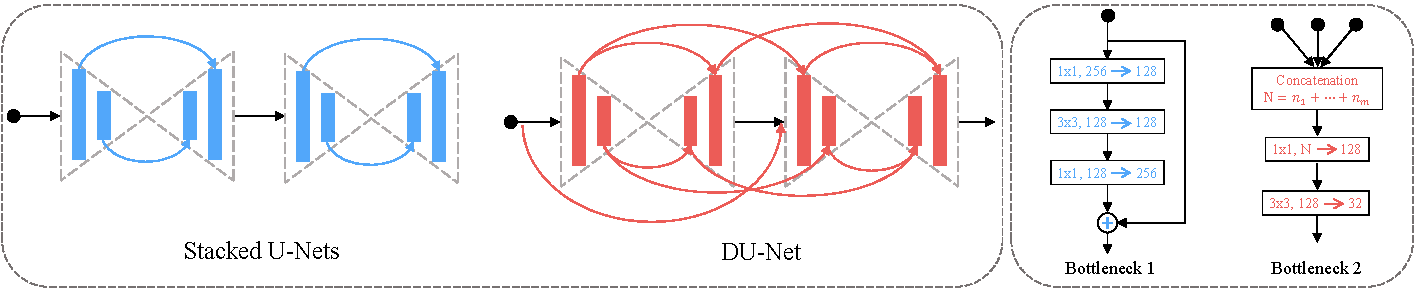
\includegraphics[width=1.0\linewidth]{figures/framework-cropped.pdf}
\caption{Illustration of stacked U-Nets and DU-Net. Stacked U-Nets has skip connections only within each U-Net. In contrast, DU-Net also connects blocks with the same semantic meanings across different U-Nets. The feature reuse could significantly reduce the size of bottleneck in each block, as shown in the right figure. Consequently, with the same number of U-Nets, DU-Net has only 30\% parameters of stacked U-Nets.}
\label{fig:framework}
\end{figure*}

% 
Our solution to those efficiency issues is threefold. {\bf First}, instead of connecting all stacked U-Nets, we only connect a U-Net to its $K$ successors. We name it as the $order$-$K$ connectivity, which aims to balance the fitting accuracy and parameter efficiency by cutting off long-distance connections. {\bf Second}, we employ a memory-efficient implementation in training. The key idea is to reuse a pre-allocated memory so all connected blocks could share the same memory. Compared with the naive implementation, this strategy makes it possible to train a very deep DU-Net (actually, $2\times$ deeper). {\bf Third}, to further improve the efficiency, we investigate an iterative design that may reduce the model size to one half. More specifically, the output of the first pass of the DU-Net is used as the input of the second pass, where detection or regression loss is applied as supervision. 

% %G%
% In view of deploying our approach on mobile devices, we further attempt to quantize weights, inputs, and gradients of DU-Net to low bit-width discrete values. This not only decreases the high precision operations but also shrinks the memory usage during training. By network quantization, the size of trained model can also be largely compressed.
% %G%
Besides shrinking the number of network parameters, we also study to further quantize each parameter. This motivates from the ubiquitous mobile applications. Although current mobile devices could carry models of dozens of MBs, deploying such networks requires high-end GPUs. However, quantized models could be accelerated by some specifically designed low-cost hardwares. Beyond only deploying models on mobile devices \cite{li2017deeprebirth}, training deep neural networks on distributed mobile devices emerges recently \cite{mcmahan2016communication}. To this end, we also try to quantize not only the model parameters but also its inputs (intermediate features) and gradients in training. This is the first attempt to investigate training landmark localizers using quantized inputs and gradients.


In summary, our key contributions are:
\begin{itemize}
    \item To the best of our knowledge, we are the first to propose quantized densely connected U-Nets for visual landmark localization, which largely improves the information flow and feature reuse at the semantic level.
    \item We propose the $order$-$K$ connectivity to balance accuracy and efficiency. It decreases the growth of model size from quadratic to linear by removing trivial connections. Experiments show it could reduce $\sim$70\% parameters of state-of-the-art landmark localizers.
    \item Very deep U-Nets can be trained using a memory-efficient implementation, where pre-allocated memory is reused by all connected blocks.
    \item We further investigate an iterative refinement that may cut down half of the model size, by forwarding DU-Net twice using either detection or regression supervision.
    %G%
    \item Different from previous efforts of quantizing only the model parameters, we are the first to quantize their inputs and gradients for better training efficiency on landmark localization tasks. By choosing appropriate quantization bit-widths for weights, inputs and gradients, quantized DU-Net achieves $\sim$75\% training memory saving with comparable performance. 
    %G%
    \item Exhaustive experiments are performed to validate DU-Net in different aspects. In both human pose estimation and face alignment, DU-Net demonstrates comparable localization accuracy and use $\sim$2\% model size compared with state-of-the-art methods.
\end{itemize}

% We are the first to deploy network quantization for better training efficiency on localization tasks. By choosing appropriate quantization bit-widths for weights, inputs and gradients, quantized DU-Net achieves at least 32$\times$ memory saving with comparable performance to the-state-of-art approaches. 


%The landmark localization such as human pose estimation \cite{toshev2014deeppose,newell2016stacked,wei2016convolutional}, facial landmark localization \cite{xiong2013supervised,zhang2014facial,sagonas2013300}, etc, plays an important role in the higher-level image understanding. The Convolutional Neural Networks (CNNs) have dominated this field, among which recent architecture of stacked hourglasses \cite{newell2016stacked}, a variant of the U-Net \cite{ronneberger2015unet}, becomes a standard solution. The skip connections between top-down and bottom-up blocks within a U-Net could preserve the spatial information and increase the gradient flow. With multiple U-Nets stacked together, the prediction could be refined stage by stage. However, the connections are only within each U-Net of the stacked hourglasses and no explicit connections exist between U-Nets, which may impede the information flow across them. And the blocks with the same semantics in different U-Nets cannot share features, leading to many redundant parameters. 

% Its success attributes to three key factors: repeated top-down, bottom-up inferences, intermediate supervisions and residual bottlenecks \cite{}. 

% The multiple stage top-down and bottom-up processing could better integrate both the local and global visual contexts into the final prediction. The intermediate supervision and residual bottlenecks, on the other hand, could alleviate the gradient vanish problem in deep networks.
%In this paper, we propose to densely connect stacked U-Nets by linking blocks with the same semantics in different U-Nets. We refer to this architecture as {\it Dense U-Nets}. The blocks in a U-Net could get direct inputs from its connected blocks in all preceding U-Nets, making the information flow more efficiently among the U-Nets. The feature reuse at each resolution could reduce the parameters in each block. The dense connectivity in our Dense U-Nets is different from that of DenseNet \cite{huang2016densely}. More specifically, layers only within each single block of the DenseNet are connected. In contrast, we connect blocks lying across the whole Dense U-Nets and connections of hierarchical blocks are mixed together. An illustration is given in Figure \ref{fig:framework}. We name it as the {\it global dense connectivity} to differentiate from the local one in the DenseNet.

% Besides, features in the Dense U-Nets are fused by the concatenation which could facilitate the information flow compared with the summation operation in the stacked hourglasses.

% Although the dense connectivity in our Dense U-Nets is similar with that of DenseNet \cite{}, 
% More recently, the DenseNet \cite{} achieves superior image classification performance over the ResNet \cite{} in terms of both the accuracy and model size, which benefits from the dense connections between layers. Its key insight is the feature reuse between layers of the same resolutions. The dense connectivity in the DenseNet, existing within one block, is local. By extending this principle, we propose a global dense connectivity, in contrast to the local connectivity in \cite{}, that blocks at the same locations of different U-Nets are connected. Hence, we refer to this architecture as {\it Dense U-Nets}. To our best knowledge, we are the first to generalize the local dense connectivity into the stacked U-Nets. 
% The global dense connectivity could make it easier to train much deeper stacked U-Nets.

% This motivates us to replace the residual modules  in the stacked hourglasses with the dense connected layers. However, this dense connectivity exists only locally within a contiguous  block in which all feature maps have the same spatial resolution. A U-Net, on the other hand, consists of a sequence of top-down and bottom-up blocks. A straight way is to turn each block into a dense block with multiple layers. However, this would sacrifice the spirit of stacked hourglasses that multiple stacked hourglasses outperform a single hourglass with multiple layers in each block.

% In order to integrate the structure of stacked U-Nets together with the idea of dense connectivity, we propose a global dense connectivity, in contrast to the local connectivity in \cite{}, that blocks at the same locations of different U-Nets are connected. Hence, we refer to this architecture as {\it Dense U-Nets}. The connected layers in the Dense U-Nets distribute along the whole network rather than in local continuous blocks. Compared with the local residual modules in the stacked hourglasses, the global dense connections could significantly facilitate the gradient to flow across stacked U-Nets.

%In practice, the Dense U-Nets have the efficiency problems of both parameter and training memory. First, suppose a Dense U-Nets contains $n$ U-Nets, there would be $O(n(n-1)/2)$ connections. Even though we use the dense bottleneck in Figure \ref{fig:framework}, the number of conv($1\times 1$) parameters still has the quadratic growth. Inspired from the Variable Order Markov (VOM) models \cite{begleiter2004prediction}, we propose the order-K connectivity that, instead of linking all the U-Nets, we connect only a fixed number of U-Nets. The goal is to use the minimum connections achieving the most obvious improvements. The multiple intermediate supervisions in the Dense U-Nets are good compensates for the order-K connectivity since they could provide additional gradients. The DenseNet does not have this advantage since it has only one supervision at the end.

% Furthermore, different from the DenseNet with only one supervision, the Dense U-Nets have multiple intermediate supervisions. The global dense connections plus the intermediate supervisions could bring faster convergence on the training set, but also gives rise to the concern of overfitting. Inspired from the Variable Order Markov (VOM) models \cite{}, we propose the order-K connectivity that, instead of linking all the U-Nets, we connect only a fixed number of U-Nets. The goal is to use the minimum connections achieving the most obvious improvement. Another advantage of order-K connectivity is that it has fewer parameters compared with the dense connectivity.

%Benefiting from the order-K connectivity, the Dense U-Nets could achieve comparable performance of stacked hourglasses with only one-third parameters. However, a naive implementation of the order-K connectivity could make the training very memory expensive. Therefore, we employ the memory efficient implementation \cite{pleiss2017memory}. The key idea is to share memories for time efficient operations such as concatenation and batch norm \cite{ioffe2015batch} within the connected layers. By pre-allocating a fixed memory, the later features produced by these operations would replace earlier features. So we need to re-compute those replaced features in the backward phase. The memory efficient implementation makes it possible to train Dense U-Nets two times deeper than the stacked hourglasses. 

%Furthermore, we also investigate to use the iterative refinement improving the parameter efficiency. Given a Dense U-Nets, we compare its performance with another Dense U-Nets with only half depth but an additional iteration. Besides, both detection and regression losses \cite{bulat2016human} were used in the landmark detection tasks, but there is no investigation yet about how they independently and collaboratively affect the prediction. We will give their detailed comparison in our experiments.

%In summary, the key contributions are:
%\begin{itemize}
%    \item To our best knowledge, we are the first to use the dense connectivity among the stacked U-Nets. The global dense connectivity in our Dense U-Nets is different from the local one in the DenseNet \cite{huang2016densely}.
%    \item We propose the order-K connectivity to make the Dense U-Nets parameter efficient. The order-K connectivity could decrease the growth of conv($1\times 1$) parameters from quadratic to linear. With comparable performance as the stacked hourglasses \cite{newell2016stacked}, it makes the Dense U-Nets require only one-third parameters. 
%    \item The memory efficient implementation of Dense U-Nets is provided to reduce its training memory usage. It makes it possible to train Dense U-Nets two times deeper than the stacked hourglasses.
%    \item We further explore using iterative refinement to improvement the parameter efficiency. At the same time, we investigate how different combinations of the detection and regression losses affect the performance.
%\end{itemize}
This section describes the training regime for our models. 

%In order to speed up experimentation, our ablations are performed relative to a smaller base model described in detail in Section \ref{sec:results}.

\subsection{Training Data and Batching}
We trained on the standard WMT 2014 English-German dataset consisting of about 4.5 million sentence pairs.  Sentences were encoded using byte-pair encoding \citep{DBLP:journals/corr/BritzGLL17}, which has a shared source-target vocabulary of about 37000 tokens. For English-French, we used the significantly larger WMT 2014 English-French dataset consisting of 36M sentences and split tokens into a 32000 word-piece vocabulary \citep{wu2016google}.  Sentence pairs were batched together by approximate sequence length.  Each training batch contained a set of sentence pairs containing approximately 25000 source tokens and 25000 target tokens.  

\subsection{Hardware and Schedule}

We trained our models on one machine with 8 NVIDIA P100 GPUs.  For our base models using the hyperparameters described throughout the paper, each training step took about 0.4 seconds.  We trained the base models for a total of 100,000 steps or 12 hours.  For our big models,(described on the bottom line of table \ref{tab:variations}), step time was 1.0 seconds.  The big models were trained for 300,000 steps (3.5 days).

\subsection{Optimizer} We used the Adam optimizer~\citep{kingma2014adam} with $\beta_1=0.9$, $\beta_2=0.98$ and $\epsilon=10^{-9}$.  We varied the learning rate over the course of training, according to the formula:

\begin{equation}
lrate = \dmodel^{-0.5} \cdot
  \min({step\_num}^{-0.5},
    {step\_num} \cdot {warmup\_steps}^{-1.5})
\end{equation}

This corresponds to increasing the learning rate linearly for the first $warmup\_steps$ training steps, and decreasing it thereafter proportionally to the inverse square root of the step number.  We used $warmup\_steps=4000$.

\subsection{Regularization} \label{sec:reg}

We employ three types of regularization during training: 
\paragraph{Residual Dropout} We apply dropout \citep{srivastava2014dropout} to the output of each sub-layer, before it is added to the sub-layer input and normalized.   In addition, we apply dropout to the sums of the embeddings and the positional encodings in both the encoder and decoder stacks.  For the base model, we use a rate of $P_{drop}=0.1$.

% \paragraph{Attention Dropout} Query to key attentions are structurally similar to hidden-to-hidden weights in a feed-forward network, albeit across positions. The softmax activations yielding attention weights can then be seen as the analogue of hidden layer activations. A natural possibility is to extend dropout \citep{srivastava2014dropout} to attention. We implement attention dropout by dropping out attention weights as,
% \begin{equation*}
%   \mathrm{Attention}(Q, K, V) = \mathrm{dropout}(\mathrm{softmax}(\frac{QK^T}{\sqrt{d}}))V
% \end{equation*}
% In addition to residual dropout, we found attention dropout to be beneficial for our parsing experiments.  

%\paragraph{Symbol Dropout} In the source and target embedding layers, we replace a random subset of the token ids with a sentinel id.  For the base model, we use a rate of $symbol\_dropout\_rate=0.1$.  Note that this applies only to the auto-regressive use of the target ids - not their use in the cross-entropy loss. 

%\paragraph{Attention Dropout} Query to memory attentions are structurally similar to hidden-to-hidden weights in a feed-forward network, albeit across positions. The softmax activations yielding attention weights can then be seen as the analogue of hidden layer activations. A natural possibility is to extend dropout \citep{srivastava2014dropout} to attentions. We implement attention dropout by dropping out attention weights as,
%\begin{equation*}
%   A(Q, K, V) = \mathrm{dropout}(\mathrm{softmax}(\frac{QK^T}{\sqrt{d}}))V
%\end{equation*}
%As a result, the query will not be able to access the memory values at the dropped out position. In our experiments, we tried attention dropout rates of 0.2, and 0.3, and found it to work favorably for English-to-German translation.
%$attention\_dropout\_rate=0.2$.

\paragraph{Label Smoothing} During training, we employed label smoothing of value $\epsilon_{ls}=0.1$ \citep{DBLP:journals/corr/SzegedyVISW15}.  This hurts perplexity, as the model learns to be more unsure, but improves accuracy and BLEU score.

%
\section{Model Fitting}
\label{sec:fitting}

We propose to fit the 3DMM on an input image using Gauss-Newton iterative
optimization. To this end, herein, we first formulate the cost function and
then present two optimization procedures.

%
%
%
\subsection{Cost Function}
The overall cost function of the proposed 3DMM formulation consists of a
texture-based term, an optional error term based on sparse 2D landmarks and
optional regularization terms on the parameters.

%
\textbf{Texture reconstruction cost.} The main term of the optimization problem
is the one that aims to estimate the shape, texture and camera parameters that
minimize the ${\ell_2}^2$ norm of the difference between the image feature-based texture that corresponds to the projected 2D locations of the 3D shape instance and the texture instance of the 3DMM. 
Let us denote by $\mathbf{F}=\mathcal{F}(\mathbf{I})$ the feature-based representation with $C$ channels of an input image $\mathbf{I}$ using Eq.~\ref{equ:features}. 
Then, the texture reconstruction cost is expressed as
%
\begin{equation}
\argmin_{\mathbf{p}, \mathbf{c}, \boldsymbol{\lambda}}
\left\lVert\mathbf{F}\left(\mathcal{W}(\mathbf{p},\mathbf{c})\right) - \mathcal{T}(\boldsymbol{\lambda})\right\rVert^2
\label{equ:data_cost}
\end{equation}
%
Note that $\mathbf{F}\left(\mathcal{W}(\mathbf{p},\mathbf{c})\right)\in\mathbb{R}^{CN}$ denotes
the operation of sampling the feature-based input image on the projected 2D locations of the 3D shape instance acquired by the camera model (Eq.~\ref{equ:camera_model}).

%
\textbf{Regularization.} In order to avoid over-fitting effects, we augment the
cost function with two optional regularization terms over the shape and texture
parameters. Let us denote as $\mathbf{\Sigma}_s\in\mathbb{R}^{n_s\times n_s}$
and $\mathbf{\Sigma}_t\in\mathbb{R}^{n_t\times n_t}$ the diagonal matrices with
the eigenvalues in their main diagonal for the shape and texture models,
respectively. Based on the PCA nature of the shape and texture models, it is
assumed that their parameters follow normal prior distributions, i.e.
$\mathbf{p}\sim\mathcal{N}(\mathbf{0},\mathbf{\Sigma}_s)$ and
$\boldsymbol{\lambda}\sim\mathcal{N}(\mathbf{0},\mathbf{\Sigma}_t)$.
We formulate the regularization terms as the ${\ell_2}^2$ of the
parameters' vectors weighted with the corresponding inverse eigenvalues, i.e.
%
\begin{equation}
\argmin_{\mathbf{p}, \boldsymbol{\lambda}}~c_s\left\lVert\mathbf{p}\right\rVert^2_{\mathbf{\Sigma}_s^{-1}} + c_t\left\lVert\boldsymbol{\lambda}\right\rVert^2_{\mathbf{\Sigma}_t^{-1}}
\label{equ:priors}
\end{equation}
%
where $c_s$ and $c_t$ are constants that weight the contribution of the regularization
terms in the cost function.

%
\textbf{2D landmarks cost.} In order to rapidly adapt the camera parameters in
the cost of Eq.~\ref{equ:data_cost}, we further expand the optimization problem
with the term
%
\begin{equation}
\argmin_{\mathbf{p},\mathbf{c}}~c_l\left\lVert\mathcal{W}_l(\mathbf{p},\mathbf{c}) - \mathbf{s}_l\right\rVert^2
\label{equ:landmarks_cost}
\end{equation}
%
where $\mathbf{s}_l={\left[x_1,y_1,\ldots,x_L,y_L\right]}^\mathsf{T}$ denotes a
set of $L$ sparse 2D landmark points ($L\ll N$) defined on the image coordinate
system and $\mathcal{W}_l(\mathbf{p},\mathbf{c})$ returns the $2L\times 1$ vector
of 2D projected locations of these $L$ sparse landmarks. Intuitively, this term
aims to drive the optimization procedure using the selected sparse landmarks as
anchors for which we have the optimal locations $\mathbf{s}_l$.
This optional landmarks-based cost is weighted with the constant $c_l$.

%
\textbf{Overall cost function.} The overall 3DMM cost function is formulated as
the sum of the terms in Eqs.~\ref{equ:data_cost},~\ref{equ:priors},~\ref{equ:landmarks_cost},
i.e.
%
\begin{equation}
\begin{aligned}
\argmin_{\mathbf{p},\mathbf{c},\boldsymbol{\lambda}}~& \left\lVert\mathbf{F}\left(\mathcal{W}(\mathbf{p},\mathbf{c})\right) - \mathcal{T}(\boldsymbol{\lambda})\right\rVert^2 + c_l\left\lVert\mathcal{W}_l(\mathbf{p},\mathbf{c}) - \mathbf{s}_l\right\rVert^2 +\\
& + c_s\left\lVert\mathbf{p}\right\rVert^2_{\mathbf{\Sigma}_s^{-1}} + c_t\left\lVert\boldsymbol{\lambda}\right\rVert^2_{\mathbf{\Sigma}_t^{-1}}
\label{equ:cost}
\end{aligned}
\end{equation}
%
The landmarks term as well as the regularization terms are optional and aim to
facilitate the optimization procedure in order to converge faster and to a better
minimum. Note that thanks to the proposed ``in-the-wild'' feature-based texture
model, the cost function does not include any parametric illumination model
similar to the ones in the relative literature~\cite{blanz1999morphable,blanz2003face}, which greatly
simplifies the optimization.

%
%
%
\subsection{Gauss-Newton Optimization}
Inspired by the extensive literature in Lucas-Kanade 2D image
alignment~\cite{baker2004lucas,matthews2004active,papandreou2008adaptive,tzimiropoulos2013optimization,antonakos2015feature,alabort2016unified},
we formulate a Gauss-Newton optimization framework. Specifically, given that
the camera projection model is applied on the image part of
Eq.~\ref{equ:cost}, the proposed optimization has a ``forward'' nature.

%
\textbf{Parameters update.} The shape, texture and camera parameters are updated
in an additive manner, i.e.
%
\begin{equation}
\mathbf{p}\leftarrow\mathbf{p}+\Delta\mathbf{p},~~\boldsymbol{\lambda}\leftarrow\boldsymbol{\lambda}+\Delta\boldsymbol{\lambda},~~\mathbf{c}\leftarrow\mathbf{c}+\Delta\mathbf{c}
\end{equation}
%
where $\Delta\mathbf{p}$, $\Delta\boldsymbol{\lambda}$ and $\Delta\mathbf{c}$
are their increments estimated at each fitting iteration. 
Note that in the case of the quaternion
used to parametrize the 3D rotation matrix, the update is performed as the
multiplication
%
\begin{equation}
\begin{aligned}
\mathbf{q}\leftarrow & (\Delta\mathbf{q})\mathbf{q} =
\left[\begin{array}{c}\Delta q_0\\\Delta\mathbf{q}_{1:3}\end{array}\right]
\left[\begin{array}{c}q_0\\\mathbf{q}_{1:3}\end{array}\right] = \\
& = \left[\begin{array}{c}\Delta q_0 q_0 - \Delta\mathbf{q}_{1:3}^\mathsf{T}\mathbf{q}_{1:3}\\ \Delta q_0\mathbf{q}_{1:3} + q_0\Delta\mathbf{q}_{1:3}+\Delta\mathbf{q}_{1:3}\times\mathbf{q}_{1:3}\end{array}\right]
\end{aligned}
\end{equation}
%
However, we will still denote it as an addition for simplicity. Finally, we found that it is beneficial to keep the focal length constant in most cases, due to its ambiguity with $t_z$.


%
\textbf{Linearization.} By introducing the additive incremental updates on the
parameters of Eq.~\ref{equ:cost}, the cost function is expressed as
%
\begin{equation}
\begin{aligned}
\argmin_{\Delta\mathbf{p},\Delta\mathbf{c},\Delta\boldsymbol{\lambda}}~& \left\lVert\mathbf{F}\left(\mathcal{W}(\mathbf{p}+\Delta\mathbf{p},\mathbf{c}+\Delta\mathbf{c})\right) - \mathcal{T}(\boldsymbol{\lambda}+\Delta\boldsymbol{\lambda})\right\rVert^2 + \\
& + c_l\left\lVert\mathcal{W}_l(\mathbf{p}+\Delta\mathbf{p},\mathbf{c}+\Delta\mathbf{c}) - \mathbf{s}_l\right\rVert^2 +\\
& + c_s\left\lVert\mathbf{p}+\Delta\mathbf{p}\right\rVert^2_{\mathbf{\Sigma}_s^{-1}} + c_t\left\lVert\boldsymbol{\lambda}+\Delta\boldsymbol{\lambda}\right\rVert^2_{\mathbf{\Sigma}_t^{-1}}
\end{aligned}
\label{equ:cost_with_deltas}
\end{equation}
%
Note that the texture reconstruction
and landmarks constraint terms of this cost function are non-linear due
to the camera model operation. We need to linearize them around
$(\mathbf{p}, \mathbf{c})$ using first order Taylor series expansion at
$(\mathbf{p}+\Delta\mathbf{p},\mathbf{c}+\Delta\mathbf{c})=(\mathbf{p},\mathbf{c})\Rightarrow(\Delta\mathbf{p},\Delta\mathbf{c})=\mathbf{0}$.
The linearization for the image term gives
%
\begin{equation}
\begin{aligned}
\mathbf{F}\left(\mathcal{W}(\mathbf{p}+\Delta\mathbf{p},\mathbf{c}+\Delta\mathbf{c})\right) \approx & \mathbf{F}\left(\mathcal{W}(\mathbf{p},\mathbf{c})\right) + \\
& + \mathbf{J}_{\mathbf{F},\mathbf{p}}\Delta\mathbf{p} + \mathbf{J}_{\mathbf{F},\mathbf{c}}\Delta\mathbf{c}
\end{aligned}
\label{equ:image_linearization}
\end{equation}
%
where $\mathbf{J}_{\mathbf{F},\mathbf{p}}=\nabla\mathbf{F}\left.\frac{\partial\mathcal{W}}{\partial\mathbf{p}}\right|_{\mathbf{p}=\mathbf{p}}$
and
$\mathbf{J}_{\mathbf{F},\mathbf{c}}=\nabla\mathbf{F}\left.\frac{\partial\mathcal{W}}{\partial\mathbf{c}}\right|_{\mathbf{c}=\mathbf{c}}$
are the \emph{image Jacobians} with respect to the shape and camera parameters, respectively. Note that most dense feature-extraction functions $\mathcal{F}(\cdot)$ are non-differentiable, thus we simply compute the gradient of the multi-channel feature image $\nabla\mathbf{F}$.
Similarly, the linearization on the sparse landmarks projection term gives
%
\begin{equation}
\mathcal{W}_l(\mathbf{p}+\Delta\mathbf{p},\mathbf{c}+\Delta\mathbf{c})\approx\mathcal{W}_l(\mathbf{p},\mathbf{c}) + \mathbf{J}_{\mathcal{W}_l,\mathbf{p}}\Delta\mathbf{p} + \mathbf{J}_{\mathcal{W}_l,\mathbf{c}}\Delta\mathbf{c}
\label{equ:landmarks_linearization}
\end{equation}
%
where
$\mathbf{J}_{\mathcal{W}_l,\mathbf{p}}=\left.\frac{\partial\mathcal{W}_l}{\partial\mathbf{p}}\right|_{\mathbf{p}=\mathbf{p}}$
and
$\mathbf{J}_{\mathcal{W}_l,\mathbf{c}}=\left.\frac{\partial\mathcal{W}_l}{\partial\mathbf{c}}\right|_{\mathbf{c}=\mathbf{c}}$
are the \emph{camera Jacobians}. Please refer to the supplementary material for more details on the computation of these derivatives.


%
\subsubsection{Simultaneous}
Herein, we aim to simultaneously solve for all parameters' increments.
By substituting Eqs.~\ref{equ:image_linearization} and~\ref{equ:landmarks_linearization}
in Eq.~\ref{equ:cost_with_deltas} we get
%
\begin{equation}
\begin{aligned}
&\argmin_{\Delta\mathbf{p},\Delta\mathbf{c},\Delta\boldsymbol{\lambda}}\\
&\left\lVert\mathbf{F}\left(\mathcal{W}(\mathbf{p},\mathbf{c})\right) + \mathbf{J}_{\mathbf{F},\mathbf{p}}\Delta\mathbf{p} + \mathbf{J}_{\mathbf{F},\mathbf{c}}\Delta\mathbf{c} - \mathcal{T}(\boldsymbol{\lambda}+\Delta\boldsymbol{\lambda})\right\rVert^2 + \\
&+ c_l\left\lVert\mathcal{W}_l(\mathbf{p},\mathbf{c}) + \mathbf{J}_{\mathcal{W}_l,\mathbf{p}}\Delta\mathbf{p} + \mathbf{J}_{\mathcal{W}_l,\mathbf{c}}\Delta\mathbf{c} - \mathbf{s}_l\right\rVert^2 +\\
&+ c_s\left\lVert\mathbf{p}+\Delta\mathbf{p}\right\rVert^2_{\mathbf{\Sigma}_s^{-1}} + c_t\left\lVert\boldsymbol{\lambda}+\Delta\boldsymbol{\lambda}\right\rVert^2_{\mathbf{\Sigma}_t^{-1}}
\end{aligned}
\label{equ:simultaneous_cost}
\end{equation}
%
Let us concatenate the parameters and their increments as
$\mathbf{b}={[\mathbf{p}^\mathsf{T}, \mathbf{c}^\mathsf{T}, \boldsymbol{\lambda}^\mathsf{T}]}^\mathsf{T}$
and
$\Delta\mathbf{b}={[\Delta\mathbf{p}^\mathsf{T}, \Delta\mathbf{c}^\mathsf{T}, \Delta\boldsymbol{\lambda}^\mathsf{T}]}^\mathsf{T}$.
By taking the derivative of the final linearized cost function with respect to
$\Delta\mathbf{b}$ and equalizing with zero, we get the solution
%
\begin{equation}
\mathbf{b} = -\mathbf{H}^{-1} \left(\mathbf{J}_{\mathbf{F}}^\mathsf{T}\mathbf{e}_{\mathbf{F}} + c_l\mathbf{J}_{\mathcal{W}_l}^\mathsf{T}\mathbf{e}_l + c_s\mathbf{\Sigma}_s^{-1}\mathbf{p} + c_t\mathbf{\Sigma}_t^{-1}\boldsymbol{\lambda}\right)
\end{equation}
%
where
$\mathbf{H}={\mathbf{J}_{\mathbf{F}}}^\mathsf{T}\mathbf{J}_{\mathbf{F}} + c_l{\mathbf{J}_{\mathcal{W}_l}}^\mathsf{T}\mathbf{J}_{\mathcal{W}_l} + c_s\mathbf{\Sigma}_s^{-1} + c_t\mathbf{\Sigma}_t^{-1}$
is the Hessian with
%
\begin{equation}
\begin{aligned}
\mathbf{J}_{\mathbf{F}} = &~{\left[\mathbf{J}_{\mathbf{F},\mathbf{p}}^\mathsf{T}, \mathbf{J}_{\mathbf{F},\mathbf{c}}^\mathsf{T}, -\mathbf{U}_t^\mathsf{T}\right]}^\mathsf{T}\\
\mathbf{J}_{\mathcal{W}_l} = &~{\left[\mathbf{J}_{\mathcal{W}_l,\mathbf{p}}^\mathsf{T}, \mathbf{J}_{\mathcal{W}_l,\mathbf{c}}^\mathsf{T}, \mathbf{0}_{n_t\times 2L}\right]}^\mathsf{T}
\end{aligned}
\end{equation}
%
and
%
\begin{equation}
\begin{aligned}
\mathbf{e}_{\mathbf{F}} = &~\mathbf{F}\left(\mathcal{W}(\mathbf{p},\mathbf{c})\right) - \mathcal{T}(\boldsymbol{\lambda})\\
\mathbf{e}_l = &~\mathcal{W}_l(\mathbf{p},\mathbf{c}) - \mathbf{s}_l
\end{aligned}
\end{equation}
%
are the residual terms. The computational complexity of the Simultaneous algorithm per iteration is dominated by the texture reconstruction term as
$\mathcal{O}((n_s+n_c+n_t)^3 + CN(n_s+n_c+n_t)^2)$, which in practice is too slow.



%
\subsubsection{Project-Out}
We propose to use a Project-Out optimization approach that is much faster than the Simultaneous. The main idea is to optimize on the orthogonal complement of the texture subspace which will eliminate the need to solve for the texture parameters increment at each iteration. By substituting Eqs.~\ref{equ:image_linearization} and~\ref{equ:landmarks_linearization}
into Eq.~\ref{equ:cost_with_deltas} and removing the incremental update on the
texture parameters as well as the texture parameters regularization term,
we end up with the problem
%
\begin{equation}
\begin{aligned}
\argmin_{\Delta\mathbf{p},\Delta\mathbf{c},\boldsymbol{\lambda}}~& \left\lVert\mathbf{F}\left(\mathcal{W}(\mathbf{p},\mathbf{c})\right) + \mathbf{J}_{\mathbf{F},\mathbf{p}}\Delta\mathbf{p} + \mathbf{J}_{\mathbf{F},\mathbf{c}}\Delta\mathbf{c} - \mathcal{T}(\boldsymbol{\lambda})\right\rVert^2 + \\
& + c_l\left\lVert\mathcal{W}_l(\mathbf{p},\mathbf{c}) + \mathbf{J}_{\mathcal{W}_l,\mathbf{p}}\Delta\mathbf{p} + \mathbf{J}_{\mathcal{W}_l,\mathbf{c}}\Delta\mathbf{c} - \mathbf{s}_l\right\rVert^2 +\\
& + c_s\left\lVert\mathbf{p}+\Delta\mathbf{p}\right\rVert^2_{\mathbf{\Sigma}_s^{-1}}
\end{aligned}
\label{equ:project_out_cost}
\end{equation}
%
The solution of Eq.~\ref{equ:project_out_cost} with respect to $\boldsymbol{\lambda}$ is
readily given by
%
\begin{equation}
\boldsymbol{\lambda} = {\mathbf{U}_t}^\mathsf{T} \left(\mathbf{F}(\mathcal{W}(\mathbf{p},\mathbf{c})) + \mathbf{J}_{\mathbf{F},\mathbf{p}}\Delta\mathbf{p} + \mathbf{J}_{\mathbf{F},\mathbf{c}}\Delta\mathbf{c} - \bar{\mathbf{t}}\right)
\label{equ:lambda_solution}
\end{equation}
%
By plugging Eq.~\ref{equ:lambda_solution} into Eq.~\ref{equ:project_out_cost},
we get
%
\begin{equation}
\begin{aligned}
\argmin_{\Delta\mathbf{p},\Delta\mathbf{c}}~& \left\lVert\mathbf{F}\left(\mathcal{W}(\mathbf{p},\mathbf{c})\right) + \mathbf{J}_{\mathbf{F},\mathbf{p}}\Delta\mathbf{p} + \mathbf{J}_{\mathbf{F},\mathbf{c}}\Delta\mathbf{c} - \bar{\mathbf{t}}\right\rVert^2_\mathbf{P} + \\
& + c_l\left\lVert\mathcal{W}_l(\mathbf{p},\mathbf{c}) + \mathbf{J}_{\mathcal{W}_l,\mathbf{p}}\Delta\mathbf{p} + \mathbf{J}_{\mathcal{W}_l,\mathbf{c}}\Delta\mathbf{c} - \mathbf{s}_l\right\rVert^2 +\\
& + c_s\left\lVert\mathbf{p}+\Delta\mathbf{p}\right\rVert^2_{\mathbf{\Sigma}_s^{-1}}
\end{aligned}
\label{equ:project_out_cost_2}
\end{equation}
%
where $\mathbf{P}=\mathbf{E}-\mathbf{U}_t{\mathbf{U}_t}^\mathsf{T}$ is the
orthogonal complement of the texture subspace that functions as the
``project-out'' operator with $\mathbf{E}$ denoting the $CN \times CN$ unitary matrix.
Note that in order to derive Eq.~\ref{equ:project_out_cost_2}, we use the properties
$\mathbf{P}^\mathsf{T}=\mathbf{P}$
and
$\mathbf{P}^\mathsf{T}\mathbf{P}=\mathbf{P}$. By differentiating
Eq.~\ref{equ:project_out_cost_2} and equalizing to zero, we get the solution
%
\begin{equation}
\begin{aligned}
\Delta\mathbf{p} = &~{\mathbf{H}_{\mathbf{p}}}^{-1} \left( \mathbf{J}_{\mathbf{F},\mathbf{p}}^\mathsf{T} \mathbf{P} \mathbf{e}_{\mathbf{F}} + c_l\mathbf{J}_{\mathcal{W}_l,\mathbf{p}}^\mathsf{T}\mathbf{e}_l + c_s\mathbf{\Sigma}^{-1}_s\mathbf{p}\right)\\
\Delta\mathbf{c} = &~{\mathbf{H}_{\mathbf{c}}}^{-1} \left( \mathbf{J}_{\mathbf{F},\mathbf{c}}^\mathsf{T} \mathbf{P} \mathbf{e}_{\mathbf{F}} + c_l\mathbf{J}_{\mathcal{W}_l,\mathbf{c}}^\mathsf{T}\mathbf{e}_l\right)
\end{aligned}
\label{equ:project_out_solution}
\end{equation}
%
where
%
\begin{equation}
\begin{aligned}
\mathbf{H}_{\mathbf{p}} = &~\mathbf{J}_{\mathbf{F},\mathbf{p}}^\mathsf{T}\mathbf{P}\mathbf{J}_{\mathbf{F},\mathbf{p}} + c_l\mathbf{J}_{\mathcal{W}_l,\mathbf{p}}^\mathsf{T}\mathbf{J}_{\mathcal{W}_l,\mathbf{p}} + c_s\mathbf{\Sigma}^{-1}\\
\mathbf{H}_{\mathbf{c}} = &~\mathbf{J}_{\mathbf{F},\mathbf{c}}^\mathsf{T}\mathbf{P}\mathbf{J}_{\mathbf{F},\mathbf{c}} + c_l\mathbf{J}_{\mathcal{W}_l,\mathbf{c}}^\mathsf{T}\mathbf{J}_{\mathcal{W}_l,\mathbf{c}}
\end{aligned}
\end{equation}
%
are the Hessian matrices and
%
\begin{equation}
\begin{aligned}
\mathbf{e}_{\mathbf{F}} = &~\mathbf{F}\left(\mathcal{W}(\mathbf{p},\mathbf{c})\right) - \bar{\mathbf{t}}\\
\mathbf{e}_l = &~\mathcal{W}_l(\mathbf{p},\mathbf{c}) - \mathbf{s}_l
\end{aligned}
\end{equation}
%
are the residual terms. The texture parameters can be estimated at the end of the iterative procedure using Eq.~\ref{equ:lambda_solution}. 

Note that the most expensive operation is $\mathbf{J}_{\mathbf{F},\mathbf{p}}^\mathsf{T}\mathbf{P}$. However, if we first do $\mathbf{J}_{\mathbf{F},\mathbf{p}}^\mathsf{T}\mathbf{U}_t$ and then multiply this result with $\mathbf{U}_t^\mathsf{T}$, the total cost becomes $\mathcal{O}(CNn_tn_s)$. The same stands for $\mathbf{J}_{\mathbf{F},\mathbf{c}}^\mathsf{T}\mathbf{P}$. Consequently, the cost per iteration is 
$\mathcal{O}((n_s+n_c)^3 + CNn_t(n_s+n_c) + CN(n_s+n_c)^2)$
which is much faster than the Simultaneous algorithm.


%
%
%
\textbf{Residual masking.}
In practice, we apply a mask on the texture reconstruction residual of the Gauss-Newton optimization, in order to speed-up the 3DMM fitting. This mask is constructed by first acquiring the set of visible vertexes using z-buffering and then randomly selecting $K$ of them. By keeping the number of vertexes small ($K\approx 5000 \ll N$), we manage to greatly speed-up the fitting process without any accuracy penalty.

\section{Training dataset}
\label{sec:dataset}
%
In this section we briefly summarize the tightly-coupled BoW and SfM reconstruction system~\cite{SRCF15,RSJFCM16} that is employed to automatically select our training data. 
Then, we describe how we exploit the 3D information to select harder matching pairs and hard non-matching pairs with larger variability. 

\subsection{BoW and 3D reconstruction}
%
The retrieval engine used in the work of Schonberger \etal~\cite{SRCF15} builds upon BoW with fast spatial verification~\cite{PCISZ07}. 
It uses Hessian affine local features~\cite{MTSZMSKG05}, \mbox{RootSIFT} descriptors~\cite{AZ12}, and a fine vocabulary of 16M visual words~\cite{MPCM13}.
Then, query images are chosen via min-hash and spatial verification, as in~\cite{CM10a}. 
Image retrieval based on BoW is used to collect images of the objects/landmarks.
These images serve as the initial matching graph for the succeeding SfM reconstruction, which is performed using state-of-the-art SfM~\cite{FGGJR10,AFSS+11}. Different mining techniques, \eg zoom in, zoom out~\cite{MCM13,MRCM14}, sideways crawl~\cite{SRCF15}, help to build larger and complete model. 

In this work, we exploit the outcome of such a system. 
Given a large unannotated image collection, images are clustered and a 3D model is constructed per cluster.
We use the terms \emph{3D model}, \emph{model} and \emph{cluster} interchangeably.
For each image, the estimated camera position is known, as well as the local features registered on the 3D model. 
We drop redundant (overlapping) 3D models, that might have been constructed from different seeds.
Models reconstructing the same landmark but from different and disjoint viewpoints are considered as non-overlapping.

\subsection{Selection of training image pairs}

A 3D model is described as a bipartite visibility graph $\bG = (\cI \cup \cP,\cE)$~\cite{LSH10}, where images $\cI$ and points $\cP$ are the vertices of the graph. 
Edges of this graph are defined by visibility relations between cameras and points, \ie if a point $p\in \cP$ is visible in an image $i\in \cI$, then there exists an edge $(i,p) \in \cE$. 
The set of points observed by an image $i$ is given by
%
\begin{equation}
\label{equ:observed_points}
\cP(i) = \{ p \in \cP: (i,p) \in \cE \}.
\end{equation} 
%

We create a dataset of tuples $\left(q, m(q), \cN(q)\right)$, where $q$ represents a query image, $m(q)$ is a positive image that matches the query, and $\cN(q)$ is a set of negative images that do not match the query.
These tuples are used to form training image pairs, where each tuple corresponds to $|\cN(q)|+1$ pairs. 
For a query image $q$, a pool $\cM(q)$ of candidate positive images is constructed based on the camera positions in the cluster of $q$.
It consists of the $k$ images with closest camera centers to the query.
Due to the wide range of camera orientations, these do not necessarily depict the same object. 
We therefore propose three different ways to sample the positive image.
The positives examples are fixed during the whole training process for all three strategies.
%

\paragraph{Positive images: MAC distance.} 
The image that has the lowest MAC distance to the query is chosen as positive, formally
%
\begin{equation}
m_1(q) = \argmin_{i \in \cM(q)} ||\mac(q)-\mac(i)||.
\label{equ:mac_pos}
\end{equation} 
%
This strategy is similar to the one followed by Arandjelovic \etal~\cite{AGTPS15}. 
They adopt this choice since only GPS coordinates are available and not camera orientations.
Downside of this approach is that the chosen matching examples already have low distance, thus not forcing network to learn much out of the positive samples.


\paragraph{Positive images: maximum inliers.} 
%
In this approach, the 3D information is exploited to choose the positive image, independently of the CNN descriptor. In particular, the image that has the highest number of co-observed 3D points with the query is chosen.
That is, 
%
\begin{equation}
\label{equ:ninl_pos}
m_2(q) = \argmax_{i \in \cM(q)} |\cP(q) \cap \cP(i)|.
\end{equation} 
%
This measure corresponds to the number of spatially verified features between two images, a measure commonly used for ranking in BoW-based retrieval. As this choice is independent of the CNN representation, it delivers more challenging positive examples.
%

%
\begin{figure}[t]
% \vspace{10pt}
\centering

\def\imheight{1.1}
\def\qnumone{1021}
\def\qnumtwo{1441}
\def\qnumthree{2461}
\def\qnumfour{6511}
\def\qnumfive{3481}
\def\qnumsix{3991}
\def\qnumseven{1111}
\def\qnumeight{5311}

\def\vnum{5}
\def\raisenum{0}

\setlength{\fboxsep}{0pt}%
\setlength{\fboxrule}{2pt}%

\setlength\tabcolsep{1.5mm}

\begin{tabular}{lclc}
% \hline
\fcolorbox{green}{black}{\includegraphics[height=\imheight cm]{fig/positives/q\qnumone.jpg}} &
\includegraphics[height=\imheight cm]{fig/positives/q\qnumone_p1.jpg} 
\includegraphics[height=\imheight cm]{fig/positives/q\qnumone_p2.jpg} 
\includegraphics[height=\imheight cm]{fig/positives/q\qnumone_p3.jpg}
% \hline
&
\fcolorbox{green}{black}{\includegraphics[height=\imheight cm]{fig/positives/q\qnumtwo.jpg}} &
\includegraphics[height=\imheight cm]{fig/positives/q\qnumtwo_p1.jpg} 
\includegraphics[height=\imheight cm]{fig/positives/q\qnumtwo_p2.jpg} 
\includegraphics[height=\imheight cm]{fig/positives/q\qnumtwo_p3.jpg}
\\
\fcolorbox{green}{black}{\includegraphics[height=\imheight cm]{fig/positives/q\qnumthree.jpg}} & 
\includegraphics[height=\imheight cm]{fig/positives/q\qnumthree_p1.jpg} 
\includegraphics[height=\imheight cm]{fig/positives/q\qnumthree_p2.jpg} 
\includegraphics[height=\imheight cm]{fig/positives/q\qnumthree_p3.jpg}
&
\fcolorbox{green}{black}{\includegraphics[height=\imheight cm]{fig/positives/q\qnumfour.jpg}} & 
\includegraphics[height=\imheight cm]{fig/positives/q\qnumfour_p1.jpg} 
\includegraphics[height=\imheight cm]{fig/positives/q\qnumfour_p2.jpg} 
\includegraphics[height=\imheight cm]{fig/positives/q\qnumfour_p3.jpg}
\\
\fcolorbox{green}{black}{\includegraphics[height=\imheight cm]{fig/positives/q\qnumfive.jpg}} & 
\includegraphics[height=\imheight cm]{fig/positives/q\qnumfive_p1.jpg} 
\includegraphics[height=\imheight cm]{fig/positives/q\qnumfive_p2.jpg} 
\includegraphics[height=\imheight cm]{fig/positives/q\qnumfive_p3.jpg}
&
\fcolorbox{green}{black}{\includegraphics[height=\imheight cm]{fig/positives/q\qnumsix.jpg}} & 
\includegraphics[height=\imheight cm]{fig/positives/q\qnumsix_p1.jpg} 
\includegraphics[height=\imheight cm]{fig/positives/q\qnumsix_p2.jpg} 
\includegraphics[height=\imheight cm]{fig/positives/q\qnumsix_p3.jpg}
\\
\fcolorbox{green}{black}{\includegraphics[height=\imheight cm]{fig/positives/q\qnumseven.jpg}} & 
\includegraphics[height=\imheight cm]{fig/positives/q\qnumseven_p1.jpg} 
\includegraphics[height=\imheight cm]{fig/positives/q\qnumseven_p2.jpg} 
\includegraphics[height=\imheight cm]{fig/positives/q\qnumseven_p3.jpg}
&
\fcolorbox{green}{black}{\includegraphics[height=\imheight cm]{fig/positives/q\qnumeight.jpg}} & 
\includegraphics[height=\imheight cm]{fig/positives/q\qnumeight_p1.jpg} 
\includegraphics[height=\imheight cm]{fig/positives/q\qnumeight_p2.jpg} 
\includegraphics[height=\imheight cm]{fig/positives/q\qnumeight_p3.jpg}
\\

\end{tabular}
\caption{Examples of training query images (green border) and matching images selected as positive examples by methods (from left to right) $m_1(q)$, $m_2(q)$, and $m_3(q)$.
\label{fig:positives}}
\end{figure}

%

\paragraph{Positive images: relaxed inliers.}
%
Even though both previous methods choose positive images depicting the same object as the query, the variance of viewpoints is limited.
Instead of using a pool of images with similar camera position, the positive example is selected at random from a set of images that co-observe enough points with the query, but do not exhibit too extreme scale change. 
The positive example in this case is  
\begin{equation}
\label{equ:relaxed_pos}
m_3(q) = \texttt{random}\left\{ i \in \cM(q): \frac{|\cP(i) \cap \cP(q)|}{|\cP(q)|} \geq t_i,~\texttt{scale}(i,q) \leq t_s \right\},
\end{equation} 
%
where $\texttt{scale}(i,q)$ is the scale change between the two images.
This method results in selecting harder matching examples which are still guaranteed to depict the same object. Method $m_3$ chooses different image than $m_1$ on 86.5\% of the queries.
In Figure~\ref{fig:positives} we present examples of query images and the corresponding positives selected with the three different methods. The relaxed method increases the variability of viewpoints. 
%

\paragraph{Negative images.} 
%
Negative examples are selected from clusters different than the cluster of the query image, as the clusters are non-overlaping. 
Following a well-known procedure, we choose hard negatives~\cite{STFKM14,GDDM14}, that is, non-matching images with the most similar descriptor. Two different strategies are proposed. In the first, $\cN_1(q)$, k-nearest neighbors from all non-matching images are selected. In the other, $\cN_2(q)$, the same criterion is used, but at most one image per cluster is allowed. While $\cN_1(q)$ often leads to multiple, and very similar, instances of the same object, $\cN_2(q)$ provides higher variability of the negative examples, see Figure~\ref{fig:negatives}. While positives examples are fixed during the whole training process, hard negatives depend on the current CNN parameters and are re-mined multiple times per epoch. 

%
\setlength{\fboxsep}{0pt}%
\setlength{\fboxrule}{2pt}%

\begin{figure}[t]
% \vspace{10pt}
\centering

\def\imheight{1cm}
\def\qnumone{253}
\def\qnumtwo{1611}
\def\qnumthree{1609}

\hspace{-10pt}

\setlength\tabcolsep{2mm}
% \def\arraystretch{1.2}

\begin{tabular}{cccc}

% \hline

\fcolorbox{green}{black}{\includegraphics[height=\imheight]{fig/negatives/q\qnumone.jpg}} &
\includegraphics[height=\imheight]{fig/negatives/q\qnumone_m2_n1.jpg} &
\foreach \neg in {2,3}  { 
	\includegraphics[height=\imheight]{fig/negatives/q\qnumone_m2_n\neg.jpg}
} $\ldots$& 
\foreach \neg in {4,5}  { 
	\includegraphics[height=\imheight]{fig/negatives/q\qnumone_m1_n\neg.jpg}
}$\ldots$\\

% \hline

\fcolorbox{green}{black}{\includegraphics[height=\imheight]{fig/negatives/q\qnumtwo.jpg}} &
\includegraphics[height=\imheight]{fig/negatives/q\qnumtwo_m2_n1.jpg} &
\foreach \neg in {3,4}  { 
	\includegraphics[height=\imheight]{fig/negatives/q\qnumtwo_m2_n\neg.jpg}
}$\ldots$ & 
\foreach \neg in {2,5}  { 
	\includegraphics[height=\imheight]{fig/negatives/q\qnumtwo_m1_n\neg.jpg}
}$\ldots$\\

% \hline

\fcolorbox{green}{black}{\includegraphics[height=\imheight]{fig/negatives/q\qnumthree.jpg}} &
\includegraphics[height=\imheight]{fig/negatives/q\qnumthree_m2_n1.jpg} &
\foreach \neg in {2,3,4}  { 
	\includegraphics[height=\imheight]{fig/negatives/q\qnumthree_m2_n\neg.jpg}
}$\ldots$ & 
\foreach \neg in {2,3,4}  { 
	\includegraphics[height=\imheight]{fig/negatives/q\qnumthree_m1_n\neg.jpg}
}$\ldots$\\

$q$ & $n(q)$ & $\cN_1(q)$ & $\cN_2(q)$ \\

% \hline

\end{tabular}\\[-.7\baselineskip]
\vspace{5pt}
\caption{Examples of training query images $q$ (green border), hardest non-matching images $n(q)$ that are always selected as negative examples, and additional non-matching images selected as negative examples by $\cN_1(q)$ and $\cN_2(q)$ methods respectively.
\label{fig:negatives}
\vspace{10pt}}
\end{figure}

%
\section{Experiments}
\label{sect:experiments}

% \begin{figure*}
%   \centering
%   \setlength{\tabcolsep}{0pt}
%   \setlength\figurewidth{0.05\textwidth}
%   \newcommand{\example}[1]{\raisebox{-.4\height}{\includegraphics[width=\figurewidth]{./figures/domains_examples/#1}}}
%   \begin{sc}
%   \begin{tabular}{r@{\hskip 1cm} ccccccccccc}
%     MNIST \cite{LeCun98} &
%     \example{mnist_0.png} &
%     \example{mnist_1.png} &
%     \example{mnist_2.png} &
%     \example{mnist_3.png} &
%     \example{mnist_4.png} &
%     \example{mnist_5.png} &
%     \example{mnist_6.png} &
%     \example{mnist_7.png} &
%     \example{mnist_8.png} &
%     \example{mnist_9.png} &
%     \example{mnist_10.png}\\
%     MNIST ($ | \Delta | $, BG) &
%     \example{mnisti_0.png} &
%     \example{mnisti_1.png} &
%     \example{mnisti_2.png} &
%     \example{mnisti_3.png} &
%     \example{mnisti_4.png} &
%     \example{mnisti_5.png} &
%     \example{mnisti_6.png} &
%     \example{mnisti_7.png} &
%     \example{mnisti_8.png} &
%     \example{mnisti_9.png} &
%     \example{mnisti_10.png}\\
%     Syn Numbers &
%     \example{syn_0.png} &
%     \example{syn_1.png} &
%     \example{syn_2.png} &
%     \example{syn_3.png} &
%     \example{syn_4.png} &
%     \example{syn_5.png} &
%     \example{syn_6.png} &
%     \example{syn_7.png} &
%     \example{syn_8.png} &
%     \example{syn_9.png} &
%     \example{syn_10.png}\\
%     SVHN \cite{Netzer11} &
%     \example{svhn_0.png} &
%     \example{svhn_1.png} &
%     \example{svhn_2.png} &
%     \example{svhn_3.png} &
%     \example{svhn_4.png} &
%     \example{svhn_5.png} &
%     \example{svhn_6.png} &
%     \example{svhn_7.png} &
%     \example{svhn_8.png} &
%     \example{svhn_9.png} &
%     \example{svhn_10.png}\\
%     Syn Signs &
%     \example{synsgn_11.png} &
%     \example{synsgn_1.png} &
%     \example{synsgn_2.png} &
%     \example{synsgn_3.png} &
%     \example{synsgn_4.png} &
%     \example{synsgn_5.png} &
%     \example{synsgn_12.png} &
%     \example{synsgn_7.png} &
%     \example{synsgn_8.png} &
%     \example{synsgn_9.png} &
%     \example{synsgn_10.png}\\
%     GTSRB \cite{Stallkamp12} &
%     \example{gtsrb_0.png} &
%     \example{gtsrb_1.png} &
%     \example{gtsrb_2.png} &
%     \example{gtsrb_3.png} &
%     \example{gtsrb_4.png} &
%     \example{gtsrb_5.png} &
%     \example{gtsrb_6.png} &
%     \example{gtsrb_7.png} &
%     \example{gtsrb_8.png} &
%     \example{gtsrb_9.png} &
%     \example{gtsrb_10.png}\\
%     % CIFAR-10 \cite{Krizhevsky09} &
%     % \example{cifar10_0.png} &
%     % \example{cifar10_1.png} &
%     % \example{cifar10_2.png} &
%     % \example{cifar10_3.png} &
%     % \example{cifar10_4.png} &
%     % \example{cifar10_5.png} &
%     % \example{cifar10_11.png} &
%     % \example{cifar10_7.png} &
%     % \example{cifar10_8.png} &
%     % \example{cifar10_9.png} &
%     % \example{cifar10_10.png}\\
%     % STL-10 \cite{Coates11} &
%     % \example{stl10_12.png} &
%     % \example{stl10_1.png} &
%     % \example{stl10_2.png} &
%     % \example{stl10_3.png} &
%     % \example{stl10_4.png} &
%     % \example{stl10_5.png} &
%     % \example{stl10_6.png} &
%     % \example{stl10_13.png} &
%     % \example{stl10_8.png} &
%     % \example{stl10_9.png} &
%     % \example{stl10_10.png}\\
%   \end{tabular}
%   \end{sc}
%   \vskip 2.5mm
%   \caption{\todo[What to do with this figure? Add Office? Remove?]Random samples from the datasets used in the experiments. See \sect{exper_quant} for details.}
%   \label{fig:exper_domains_examples}
% \end{figure*}

\begin{figure*}
  \centering
  \setlength{\tabcolsep}{0pt}
  \setlength\figurewidth{0.05\textwidth}
  \newcommand{\example}[1]{\raisebox{-.4\height}{\includegraphics[width=\figurewidth]{./figures/domains_examples/#1}}}
  \begin{sc}
  \begin{small}
  \begin{tabular}{r@{\hskip 0.5cm} ccc c@{\hskip 0.4cm} ccc c@{\hskip 0.4cm} ccc c@{\hskip 0.4cm} ccc}
    &
    \multicolumn{3}{c}{MNIST} & &
    \multicolumn{3}{c}{Syn Numbers} & &
    \multicolumn{3}{c}{SVHN} & &
    \multicolumn{3}{c}{Syn Signs}\\
    
    Source &
    \example{mnist_0.png} &
    \example{mnist_1.png} &
    \example{mnist_3.png} & &
    
    \example{syn_0.png} &
    \example{syn_1.png} &
    \example{syn_2.png} & &
    
    \example{svhn_3.png} &
    \example{svhn_4.png} &
    \example{svhn_5.png} & &
    
    \example{synsgn_3.png} &
    \example{synsgn_4.png} &
    \example{synsgn_5.png}\\
    
    Target &
    \example{mnisti_0.png} &
    \example{mnisti_1.png} &
    \example{mnisti_2.png} & &
    
    \example{svhn_0.png} &
    \example{svhn_1.png} &
    \example{svhn_2.png} & &
    
    \example{mnist_4.png} &
    \example{mnist_5.png} &
    \example{mnist_6.png} & &
    
    \example{gtsrb_2.png} &
    \example{gtsrb_3.png} &
    \example{gtsrb_4.png}\\
    
    &
    \multicolumn{3}{c}{\rule{0pt}{0.35cm} MNIST-M} & &
    \multicolumn{3}{c}{SVHN} & &
    \multicolumn{3}{c}{MNIST} & &
    \multicolumn{3}{c}{GTSRB}\\
  \end{tabular}
  \end{small}
  \end{sc}
  \caption{Examples of domain pairs used in the experiments. See \sect{exper_quant} for details.}
  \label{fig:exper_domains_examples}
\end{figure*}


\begin{table*}[t]
  \vskip 0.15in
  \begin{center}
    \begin{small}
      \begin{sc}
        \renewcommand{\arraystretch}{1.5}
        \begin{tabular}{l r | c c c c}
          \hline
          \multirow{2}{*}{Method} & {\scriptsize Source} & MNIST & Syn Numbers & SVHN & Syn Signs \\
          & {\scriptsize Target} & MNIST-M & SVHN & MNIST & GTSRB \\
          \hline
          \multicolumn{2}{l |}{Source only} & 
          $ .5749 $                      & $ .8665 $                      & $ .5919 $                      & $ .7400 $                      \\
          \multicolumn{2}{l |}{SA \cite{Fernando13}} & 
          $ .6078 \; (7.9\%) $           & $ .8672 \; (1.3\%) $           & $ .6157 \; (5.9\%) $           & $ .7635 \; (9.1\%) $           \\
          \multicolumn{2}{l |}{Proposed approach} & 
          $ \mathbf{.8149} \; (57.9\%) $ & $ \mathbf{.9048} \; (66.1\%) $ & $ \mathbf{.7107} \; (29.3\%) $ & $ \mathbf{.8866} \; (56.7\%) $ \\
          \multicolumn{2}{l |}{Train on target} & 
          $ .9891 $                      & $ .9244 $                      & $ .9951 $                      & $ .9987 $                      \\
          \hline
        \end{tabular}
      \end{sc}
    \end{small}
  \end{center}
    \caption{Classification accuracies for digit image classifications for different source and target domains. {\sc MNIST-M} corresponds to difference-blended digits over non-uniform background. The first row corresponds to the lower performance bound (i.e.\ if no adaptation is performed). The last row corresponds to training on the target domain data with known class labels (upper bound on the DA performance). For each of the two DA methods (ours and \cite{Fernando13}) we show how much of the gap between the lower and the upper bounds was covered (in brackets). For all five cases, our approach outperforms \cite{Fernando13} considerably, and covers a big portion of the gap.\vspace{-0mm} }
  \label{tab:results}
  \vskip -0.1in
\end{table*}

\begin{table*}[t]
  \vskip 0.15in
  \begin{center}
    \begin{small}
      \begin{sc}
        \renewcommand{\arraystretch}{1.5}
        \begin{tabular}{l r | c c c}
          \hline
          \multirow{2}{*}{Method} & {\scriptsize Source} & Amazon & DSLR & Webcam \\
          & {\scriptsize Target} & Webcam & Webcam & DSLR \\
          \hline
          \multicolumn{2}{l |}{GFK(PLS, PCA) \cite{Gong12}} & 
          $ .464 \pm .005 $ & $ .613 \pm .004 $ & $ .663 \pm .004 $\\ 
          \multicolumn{2}{l |}{SA \cite{Fernando13}} & 
          $ .450 $ & $ .648 $ & $ .699 $\\ 
          \multicolumn{2}{l |}{DA-NBNN \cite{Tommasi13}} & 
          $ .528 \pm .037 $ & $ .766 \pm .017 $ & $ .762 \pm .025 $\\ 
          \multicolumn{2}{l |}{DLID \cite{Chopra13}} & 
          $ .519 $ & $ .782 $ & $ .899 $\\
          \multicolumn{2}{l |}{DeCAF$_6$ Source Only \cite{Donahue14}} &
          $ .522 \pm .017 $ & $ .915 \pm .015 $ & --\\ 
          \multicolumn{2}{l |}{DaNN \cite{Ghifary14}} & 
          $ .536 \pm .002 $ & $ .712 \pm .000 $ & $ .835 \pm .000 $\\ 
          \multicolumn{2}{l |}{DDC \cite{Tzeng14}} & 
          $ .594 \pm .008 $ & $ .925 \pm .003 $ & $ .917 \pm .008 $\\ 
          \multicolumn{2}{l |}{Proposed Approach} & 
          $ \mathbf{ .673 \pm .017 } $ & $ \mathbf{ .940 \pm .008 } $ & $ \mathbf{ .937 \pm .010 } $\\
          \hline
        \end{tabular}
      \end{sc}
    \end{small}
  \end{center}
    \caption{Accuracy evaluation of different DA approaches on the standard {\sc Office} \cite{Saenko10} dataset. Our method (last row) outperforms competitors setting the new state-of-the-art.}
  \label{tab:results_office}
\end{table*}

% Other rows refer to the following algorithms (from top to bottom): Geodesic Flow Kernel \cite{Gong12}, Subspace Alignment \cite{Fernando13}, Naive Bayes Nearest Neighbor \cite{Tommasi13},  deep learning approach from \cite{Chopra13}, DeCAF$_6$-features described in \cite{Donahue14}, Domain Adaptive NNs \cite{Ghifary14}, Deep Domain Confusion \cite{Tzeng14}.

\def\X{{\mathbf X}}
\def\y{{\mathbf y}}

% \vspace{2mm}\noindent {\bf Datasets.}
% \label{sect:exper_datasets}

% In order to test our method in the setting of traffic signs classification we obtained~100,000 synthetic images ({\sc Syn~Signs}) simulating various photoshooting conditions. This dataset was used in conjunction with {\it The German Traffic Sign Recognition Benchmark} ({\sc GTSRB}) \cite{Stallkamp12}.

% Finally, we perform domain adaption for the {\sc CIFAR-10} and the {\sc STL-10} downsampled to the size of $ 32 \times 32 $. This pair is considerably different from the previously mentioned datasets as the intra-class variability here is higher.

We perform extensive evaluation of the proposed approach on a number of popular image datasets and their modifications. These include large-scale datasets of small images popular with deep learning methods, and the {\sc Office} datasets \cite{Saenko10}, which are a {\em de facto} standard for domain adaptation in computer vision, but have much fewer images.

\vspace{2mm}\noindent {\bf Baselines.} For the bulk of experiments the following baselines are evaluated. The \textbf{source-only} model is trained without consideration for target-domain data (no domain classifier branch included into the network). The \textbf{train-on-target} model is trained on the target domain with class labels revealed. This model serves as an upper bound on DA methods, assuming that target data are abundant and the shift between the domains is considerable. 

In addition, we compare our approach against the recently proposed unsupervised DA method based on \textbf{subspace alignment (SA)} \cite{Fernando13}, which is simple to setup and test on new datasets, but has also been shown to perform very well in experimental comparisons with other ``shallow'' DA methods. To boost the performance of this baseline, we pick its most important free parameter (the number of principal components) from the range $ \{ 2, \ldots, 60 \} $, so that the test performance on the target domain is maximized. To apply SA in our setting, we train a source-only model and then consider the activations of the last hidden layer in the label predictor (before the final linear classifier) as descriptors/features, and learn the mapping between the source and the target domains \cite{Fernando13}.

Since the SA baseline requires to train a new classifier after adapting the features, and in order to put all the compared settings on an equal footing, we retrain the last layer of the label predictor using a standard linear SVM~\cite{liblinear} for all four considered methods (including ours; the performance on the target domain remains approximately the same after the retraining). 

For the {\sc Office} dataset \cite{Saenko10}, we directly compare the performance of our full network (feature extractor and label predictor) against recent DA approaches using previously published results.

\vspace{2mm}\noindent {\bf CNN architectures.} In general, we compose feature extractor from two or three convolutional layers, picking their exact configurations from previous works. We give the exact architectures in \ref{sect:appendix_archs}.

For the domain adaptator we stick to the three fully connected layers ($x\rightarrow1024\rightarrow1024\rightarrow2$), except for {\sc MNIST} where we used a simpler ($x\rightarrow100\rightarrow2$) architecture to speed up the experiments.

For loss functions, we set $ L_y $ and $ L_d $ to be the logistic regression loss and the binomial cross-entropy respectively.

\vspace{2mm}\noindent {\bf CNN training procedure.}
The model is trained on $128$-sized batches. Images are preprocessed by the mean subtraction. A half of each batch is populated by the samples from the source domain (with known labels), the rest is comprised of the target domain (with unknown labels).

In order to suppress noisy signal from the domain classifier at the early stages of the training procedure instead of fixing the adaptation factor $ \lambda $, we gradually change it from $0$ to $1$ using the following schedule:
\begin{equation}
  \lambda_p = \frac{2}{1 + \exp(-\gamma \cdot p)} - 1,
\end{equation}
where $\gamma$ was set to $10$ in all experiments (the schedule was not optimized/tweaked). Further details on the CNN training can be found in \ref{sect:appendix_training}.

\vspace{2mm}\noindent {\bf Visualizations.}
We use t-SNE \cite{Maaten13} projection to visualize feature distributions at different points of the network, while color-coding the domains (\fig{exper_adapt_vis}). We observe strong correspondence between the success of the adaptation in terms of the classification accuracy for the target domain, and the overlap between the domain distributions in such visualizations.
 
\vspace{2mm}\noindent {\bf Choosing meta-parameters.} 
In general, good unsupervised DA methods should provide ways to set meta-parameters (such as $\lambda$, the learning rate, the momentum rate, the network architecture for our method) in an unsupervised way, i.e.\ without referring to labeled data in the target domain. %Here we would like to give few recommendations concerning this matter. First, as it was pointed out in \sect{theory} the domain classifier should not be significantly more complex than the label predictor. 
In our method, one can assess the performance of the whole system (and the effect of changing hyper-parameters) by observing the test error on the source domain {\em and} the domain classifier error. In general, we observed a good correspondence between the success of adaptation and these errors (adaptation is more successful when the source domain test error is low, while the domain classifier error is high).
In addition, the layer, where the the domain adaptator is attached can be picked by computing difference between means as suggested in \cite{Tzeng14}. 

% \begin{figure*}
%   \centering
%   {\sc MNIST $ \rightarrow $ MNIST ($ | \Delta | $, bg)}: top feature extractor layer
%   \setcounter{subfigure}{0}
%   \subfigure[Non-adapted]{%%
%     \scalebox{0.8}{%% Creator: Matplotlib, PGF backend
%%
%% To include the figure in your LaTeX document, write
%%   \input{<filename>.pgf}
%%
%% Make sure the required packages are loaded in your preamble
%%   \usepackage{pgf}
%%
%% Figures using additional raster images can only be included by \input if
%% they are in the same directory as the main LaTeX file. For loading figures
%% from other directories you can use the `import` package
%%   \usepackage{import}
%% and then include the figures with
%%   \import{<path to file>}{<filename>.pgf}
%%
%% Matplotlib used the following preamble
%%   \usepackage[utf8x]{inputenc}
%%   \usepackage[T1]{fontenc}
%%
\begingroup%
\makeatletter%
\begin{pgfpicture}%
\pgfpathrectangle{\pgfpointorigin}{\pgfqpoint{3.338520in}{2.040000in}}%
\pgfusepath{use as bounding box}%
\begin{pgfscope}%
\pgfsetbuttcap%
\pgfsetroundjoin%
\definecolor{currentfill}{rgb}{1.000000,1.000000,1.000000}%
\pgfsetfillcolor{currentfill}%
\pgfsetlinewidth{0.000000pt}%
\definecolor{currentstroke}{rgb}{1.000000,1.000000,1.000000}%
\pgfsetstrokecolor{currentstroke}%
\pgfsetdash{}{0pt}%
\pgfpathmoveto{\pgfqpoint{0.000000in}{-0.000000in}}%
\pgfpathlineto{\pgfqpoint{3.338520in}{-0.000000in}}%
\pgfpathlineto{\pgfqpoint{3.338520in}{2.040000in}}%
\pgfpathlineto{\pgfqpoint{0.000000in}{2.040000in}}%
\pgfpathclose%
\pgfusepath{fill}%
\end{pgfscope}%
\begin{pgfscope}%
\pgftext[at=\pgfqpoint{0.510000in}{0.348333in},left,bottom]{\pgfimage[interpolate=true,width=2.553333in,height=1.500000in]{./figures/adaptation_vis/pool2_mnist2inv_before-img0.png}}%
\end{pgfscope}%
\begin{pgfscope}%
\pgftext[at=\pgfqpoint{0.805000in}{0.383333in},left,bottom]{\pgfimage[interpolate=true,width=2.201667in,height=1.371667in]{./figures/adaptation_vis/pool2_mnist2inv_before-img1.png}}%
\end{pgfscope}%
\end{pgfpicture}%
\makeatother%
\endgroup%
}}%%
%   \subfigure[Adapted]{%%
%     \scalebox{0.8}{%% Creator: Matplotlib, PGF backend
%%
%% To include the figure in your LaTeX document, write
%%   \input{<filename>.pgf}
%%
%% Make sure the required packages are loaded in your preamble
%%   \usepackage{pgf}
%%
%% Figures using additional raster images can only be included by \input if
%% they are in the same directory as the main LaTeX file. For loading figures
%% from other directories you can use the `import` package
%%   \usepackage{import}
%% and then include the figures with
%%   \import{<path to file>}{<filename>.pgf}
%%
%% Matplotlib used the following preamble
%%   \usepackage[utf8x]{inputenc}
%%   \usepackage[T1]{fontenc}
%%
\begingroup%
\makeatletter%
\begin{pgfpicture}%
\pgfpathrectangle{\pgfpointorigin}{\pgfqpoint{3.340000in}{2.040000in}}%
\pgfusepath{use as bounding box}%
\begin{pgfscope}%
\pgfsetbuttcap%
\pgfsetroundjoin%
\definecolor{currentfill}{rgb}{1.000000,1.000000,1.000000}%
\pgfsetfillcolor{currentfill}%
\pgfsetlinewidth{0.000000pt}%
\definecolor{currentstroke}{rgb}{1.000000,1.000000,1.000000}%
\pgfsetstrokecolor{currentstroke}%
\pgfsetdash{}{0pt}%
\pgfpathmoveto{\pgfqpoint{0.000000in}{-0.000000in}}%
\pgfpathlineto{\pgfqpoint{3.340000in}{-0.000000in}}%
\pgfpathlineto{\pgfqpoint{3.340000in}{2.040000in}}%
\pgfpathlineto{\pgfqpoint{0.000000in}{2.040000in}}%
\pgfpathclose%
\pgfusepath{fill}%
\end{pgfscope}%
\begin{pgfscope}%
\pgftext[at=\pgfqpoint{0.518333in}{0.321667in},left,bottom]{\pgfimage[interpolate=true,width=2.565000in,height=1.550000in]{./figures/adaptation_vis/pool2_mnist2inv_after-img0.png}}%
\end{pgfscope}%
\begin{pgfscope}%
\pgftext[at=\pgfqpoint{0.518333in}{0.321667in},left,bottom]{\pgfimage[interpolate=true,width=2.565000in,height=1.553333in]{./figures/adaptation_vis/pool2_mnist2inv_after-img1.png}}%
\end{pgfscope}%
\end{pgfpicture}%
\makeatother%
\endgroup%
}}\\
%   \vspace{5mm}
%   {\sc Syn Numbers $ \rightarrow $ SVHN}: last hidden layer of the label predictor
%   \setcounter{subfigure}{0}
%   \subfigure[Non-adapted]{%%
%     \scalebox{0.8}{%% Creator: Matplotlib, PGF backend
%%
%% To include the figure in your LaTeX document, write
%%   \input{<filename>.pgf}
%%
%% Make sure the required packages are loaded in your preamble
%%   \usepackage{pgf}
%%
%% Figures using additional raster images can only be included by \input if
%% they are in the same directory as the main LaTeX file. For loading figures
%% from other directories you can use the `import` package
%%   \usepackage{import}
%% and then include the figures with
%%   \import{<path to file>}{<filename>.pgf}
%%
%% Matplotlib used the following preamble
%%   \usepackage[utf8x]{inputenc}
%%   \usepackage[T1]{fontenc}
%%
\begingroup%
\makeatletter%
\begin{pgfpicture}%
\pgfpathrectangle{\pgfpointorigin}{\pgfqpoint{3.340000in}{2.040000in}}%
\pgfusepath{use as bounding box}%
\begin{pgfscope}%
\pgfsetbuttcap%
\pgfsetroundjoin%
\definecolor{currentfill}{rgb}{1.000000,1.000000,1.000000}%
\pgfsetfillcolor{currentfill}%
\pgfsetlinewidth{0.000000pt}%
\definecolor{currentstroke}{rgb}{1.000000,1.000000,1.000000}%
\pgfsetstrokecolor{currentstroke}%
\pgfsetdash{}{0pt}%
\pgfpathmoveto{\pgfqpoint{0.000000in}{-0.000000in}}%
\pgfpathlineto{\pgfqpoint{3.340000in}{-0.000000in}}%
\pgfpathlineto{\pgfqpoint{3.340000in}{2.040000in}}%
\pgfpathlineto{\pgfqpoint{0.000000in}{2.040000in}}%
\pgfpathclose%
\pgfusepath{fill}%
\end{pgfscope}%
\begin{pgfscope}%
\pgftext[at=\pgfqpoint{0.491667in}{0.335000in},left,bottom]{\pgfimage[interpolate=true,width=2.618333in,height=1.531667in]{./figures/adaptation_vis/before-img0.png}}%
\end{pgfscope}%
\begin{pgfscope}%
\pgftext[at=\pgfqpoint{0.758333in}{0.331667in},left,bottom]{\pgfimage[interpolate=true,width=2.171667in,height=1.436667in]{./figures/adaptation_vis/before-img1.png}}%
\end{pgfscope}%
\begin{pgfscope}%
\pgfsetbuttcap%
\pgfsetroundjoin%
\definecolor{currentfill}{rgb}{0.000000,0.000000,1.000000}%
\pgfsetfillcolor{currentfill}%
\pgfsetfillopacity{0.300000}%
\pgfsetlinewidth{0.150562pt}%
\definecolor{currentstroke}{rgb}{0.000000,0.000000,0.000000}%
\pgfsetstrokecolor{currentstroke}%
\pgfsetstrokeopacity{0.300000}%
\pgfsetdash{}{0pt}%
\pgfpathmoveto{\pgfqpoint{2.521160in}{1.775861in}}%
\pgfpathcurveto{\pgfqpoint{2.525278in}{1.775861in}}{\pgfqpoint{2.529228in}{1.777497in}}{\pgfqpoint{2.532140in}{1.780409in}}%
\pgfpathcurveto{\pgfqpoint{2.535052in}{1.783321in}}{\pgfqpoint{2.536688in}{1.787271in}}{\pgfqpoint{2.536688in}{1.791389in}}%
\pgfpathcurveto{\pgfqpoint{2.536688in}{1.795507in}}{\pgfqpoint{2.535052in}{1.799457in}}{\pgfqpoint{2.532140in}{1.802369in}}%
\pgfpathcurveto{\pgfqpoint{2.529228in}{1.805281in}}{\pgfqpoint{2.525278in}{1.806917in}}{\pgfqpoint{2.521160in}{1.806917in}}%
\pgfpathcurveto{\pgfqpoint{2.517042in}{1.806917in}}{\pgfqpoint{2.513092in}{1.805281in}}{\pgfqpoint{2.510180in}{1.802369in}}%
\pgfpathcurveto{\pgfqpoint{2.507268in}{1.799457in}}{\pgfqpoint{2.505631in}{1.795507in}}{\pgfqpoint{2.505631in}{1.791389in}}%
\pgfpathcurveto{\pgfqpoint{2.505631in}{1.787271in}}{\pgfqpoint{2.507268in}{1.783321in}}{\pgfqpoint{2.510180in}{1.780409in}}%
\pgfpathcurveto{\pgfqpoint{2.513092in}{1.777497in}}{\pgfqpoint{2.517042in}{1.775861in}}{\pgfqpoint{2.521160in}{1.775861in}}%
\pgfpathclose%
\pgfusepath{stroke,fill}%
\end{pgfscope}%
\begin{pgfscope}%
\pgfsetbuttcap%
\pgfsetroundjoin%
\definecolor{currentfill}{rgb}{0.000000,0.000000,1.000000}%
\pgfsetfillcolor{currentfill}%
\pgfsetfillopacity{0.300000}%
\pgfsetlinewidth{0.150562pt}%
\definecolor{currentstroke}{rgb}{0.000000,0.000000,0.000000}%
\pgfsetstrokecolor{currentstroke}%
\pgfsetstrokeopacity{0.300000}%
\pgfsetdash{}{0pt}%
\pgfpathmoveto{\pgfqpoint{2.598938in}{1.785583in}}%
\pgfpathcurveto{\pgfqpoint{2.603056in}{1.785583in}}{\pgfqpoint{2.607006in}{1.787219in}}{\pgfqpoint{2.609918in}{1.790131in}}%
\pgfpathcurveto{\pgfqpoint{2.612830in}{1.793043in}}{\pgfqpoint{2.614466in}{1.796993in}}{\pgfqpoint{2.614466in}{1.801111in}}%
\pgfpathcurveto{\pgfqpoint{2.614466in}{1.805229in}}{\pgfqpoint{2.612830in}{1.809179in}}{\pgfqpoint{2.609918in}{1.812091in}}%
\pgfpathcurveto{\pgfqpoint{2.607006in}{1.815003in}}{\pgfqpoint{2.603056in}{1.816639in}}{\pgfqpoint{2.598938in}{1.816639in}}%
\pgfpathcurveto{\pgfqpoint{2.594819in}{1.816639in}}{\pgfqpoint{2.590869in}{1.815003in}}{\pgfqpoint{2.587957in}{1.812091in}}%
\pgfpathcurveto{\pgfqpoint{2.585045in}{1.809179in}}{\pgfqpoint{2.583409in}{1.805229in}}{\pgfqpoint{2.583409in}{1.801111in}}%
\pgfpathcurveto{\pgfqpoint{2.583409in}{1.796993in}}{\pgfqpoint{2.585045in}{1.793043in}}{\pgfqpoint{2.587957in}{1.790131in}}%
\pgfpathcurveto{\pgfqpoint{2.590869in}{1.787219in}}{\pgfqpoint{2.594819in}{1.785583in}}{\pgfqpoint{2.598938in}{1.785583in}}%
\pgfpathclose%
\pgfusepath{stroke,fill}%
\end{pgfscope}%
\begin{pgfscope}%
\pgfsetbuttcap%
\pgfsetroundjoin%
\definecolor{currentfill}{rgb}{0.000000,0.000000,1.000000}%
\pgfsetfillcolor{currentfill}%
\pgfsetfillopacity{0.300000}%
\pgfsetlinewidth{0.150562pt}%
\definecolor{currentstroke}{rgb}{0.000000,0.000000,0.000000}%
\pgfsetstrokecolor{currentstroke}%
\pgfsetstrokeopacity{0.300000}%
\pgfsetdash{}{0pt}%
\pgfpathmoveto{\pgfqpoint{2.676715in}{1.771000in}}%
\pgfpathcurveto{\pgfqpoint{2.680833in}{1.771000in}}{\pgfqpoint{2.684783in}{1.772636in}}{\pgfqpoint{2.687695in}{1.775548in}}%
\pgfpathcurveto{\pgfqpoint{2.690607in}{1.778460in}}{\pgfqpoint{2.692244in}{1.782410in}}{\pgfqpoint{2.692244in}{1.786528in}}%
\pgfpathcurveto{\pgfqpoint{2.692244in}{1.790646in}}{\pgfqpoint{2.690607in}{1.794596in}}{\pgfqpoint{2.687695in}{1.797508in}}%
\pgfpathcurveto{\pgfqpoint{2.684783in}{1.800420in}}{\pgfqpoint{2.680833in}{1.802056in}}{\pgfqpoint{2.676715in}{1.802056in}}%
\pgfpathcurveto{\pgfqpoint{2.672597in}{1.802056in}}{\pgfqpoint{2.668647in}{1.800420in}}{\pgfqpoint{2.665735in}{1.797508in}}%
\pgfpathcurveto{\pgfqpoint{2.662823in}{1.794596in}}{\pgfqpoint{2.661187in}{1.790646in}}{\pgfqpoint{2.661187in}{1.786528in}}%
\pgfpathcurveto{\pgfqpoint{2.661187in}{1.782410in}}{\pgfqpoint{2.662823in}{1.778460in}}{\pgfqpoint{2.665735in}{1.775548in}}%
\pgfpathcurveto{\pgfqpoint{2.668647in}{1.772636in}}{\pgfqpoint{2.672597in}{1.771000in}}{\pgfqpoint{2.676715in}{1.771000in}}%
\pgfpathclose%
\pgfusepath{stroke,fill}%
\end{pgfscope}%
\begin{pgfscope}%
\pgftext[x=2.798938in,y=1.762222in,left,base]{{\rmfamily\fontsize{8.000000}{9.600000}\selectfont Source}}%
\end{pgfscope}%
\begin{pgfscope}%
\pgfsetbuttcap%
\pgfsetroundjoin%
\definecolor{currentfill}{rgb}{1.000000,0.000000,0.000000}%
\pgfsetfillcolor{currentfill}%
\pgfsetfillopacity{0.300000}%
\pgfsetlinewidth{0.150562pt}%
\definecolor{currentstroke}{rgb}{0.000000,0.000000,0.000000}%
\pgfsetstrokecolor{currentstroke}%
\pgfsetstrokeopacity{0.300000}%
\pgfsetdash{}{0pt}%
\pgfpathmoveto{\pgfqpoint{2.521160in}{1.620928in}}%
\pgfpathcurveto{\pgfqpoint{2.525278in}{1.620928in}}{\pgfqpoint{2.529228in}{1.622564in}}{\pgfqpoint{2.532140in}{1.625476in}}%
\pgfpathcurveto{\pgfqpoint{2.535052in}{1.628388in}}{\pgfqpoint{2.536688in}{1.632338in}}{\pgfqpoint{2.536688in}{1.636456in}}%
\pgfpathcurveto{\pgfqpoint{2.536688in}{1.640574in}}{\pgfqpoint{2.535052in}{1.644524in}}{\pgfqpoint{2.532140in}{1.647436in}}%
\pgfpathcurveto{\pgfqpoint{2.529228in}{1.650348in}}{\pgfqpoint{2.525278in}{1.651984in}}{\pgfqpoint{2.521160in}{1.651984in}}%
\pgfpathcurveto{\pgfqpoint{2.517042in}{1.651984in}}{\pgfqpoint{2.513092in}{1.650348in}}{\pgfqpoint{2.510180in}{1.647436in}}%
\pgfpathcurveto{\pgfqpoint{2.507268in}{1.644524in}}{\pgfqpoint{2.505631in}{1.640574in}}{\pgfqpoint{2.505631in}{1.636456in}}%
\pgfpathcurveto{\pgfqpoint{2.505631in}{1.632338in}}{\pgfqpoint{2.507268in}{1.628388in}}{\pgfqpoint{2.510180in}{1.625476in}}%
\pgfpathcurveto{\pgfqpoint{2.513092in}{1.622564in}}{\pgfqpoint{2.517042in}{1.620928in}}{\pgfqpoint{2.521160in}{1.620928in}}%
\pgfpathclose%
\pgfusepath{stroke,fill}%
\end{pgfscope}%
\begin{pgfscope}%
\pgfsetbuttcap%
\pgfsetroundjoin%
\definecolor{currentfill}{rgb}{1.000000,0.000000,0.000000}%
\pgfsetfillcolor{currentfill}%
\pgfsetfillopacity{0.300000}%
\pgfsetlinewidth{0.150562pt}%
\definecolor{currentstroke}{rgb}{0.000000,0.000000,0.000000}%
\pgfsetstrokecolor{currentstroke}%
\pgfsetstrokeopacity{0.300000}%
\pgfsetdash{}{0pt}%
\pgfpathmoveto{\pgfqpoint{2.598938in}{1.630650in}}%
\pgfpathcurveto{\pgfqpoint{2.603056in}{1.630650in}}{\pgfqpoint{2.607006in}{1.632286in}}{\pgfqpoint{2.609918in}{1.635198in}}%
\pgfpathcurveto{\pgfqpoint{2.612830in}{1.638110in}}{\pgfqpoint{2.614466in}{1.642060in}}{\pgfqpoint{2.614466in}{1.646178in}}%
\pgfpathcurveto{\pgfqpoint{2.614466in}{1.650296in}}{\pgfqpoint{2.612830in}{1.654246in}}{\pgfqpoint{2.609918in}{1.657158in}}%
\pgfpathcurveto{\pgfqpoint{2.607006in}{1.660070in}}{\pgfqpoint{2.603056in}{1.661706in}}{\pgfqpoint{2.598938in}{1.661706in}}%
\pgfpathcurveto{\pgfqpoint{2.594819in}{1.661706in}}{\pgfqpoint{2.590869in}{1.660070in}}{\pgfqpoint{2.587957in}{1.657158in}}%
\pgfpathcurveto{\pgfqpoint{2.585045in}{1.654246in}}{\pgfqpoint{2.583409in}{1.650296in}}{\pgfqpoint{2.583409in}{1.646178in}}%
\pgfpathcurveto{\pgfqpoint{2.583409in}{1.642060in}}{\pgfqpoint{2.585045in}{1.638110in}}{\pgfqpoint{2.587957in}{1.635198in}}%
\pgfpathcurveto{\pgfqpoint{2.590869in}{1.632286in}}{\pgfqpoint{2.594819in}{1.630650in}}{\pgfqpoint{2.598938in}{1.630650in}}%
\pgfpathclose%
\pgfusepath{stroke,fill}%
\end{pgfscope}%
\begin{pgfscope}%
\pgfsetbuttcap%
\pgfsetroundjoin%
\definecolor{currentfill}{rgb}{1.000000,0.000000,0.000000}%
\pgfsetfillcolor{currentfill}%
\pgfsetfillopacity{0.300000}%
\pgfsetlinewidth{0.150562pt}%
\definecolor{currentstroke}{rgb}{0.000000,0.000000,0.000000}%
\pgfsetstrokecolor{currentstroke}%
\pgfsetstrokeopacity{0.300000}%
\pgfsetdash{}{0pt}%
\pgfpathmoveto{\pgfqpoint{2.676715in}{1.616066in}}%
\pgfpathcurveto{\pgfqpoint{2.680833in}{1.616066in}}{\pgfqpoint{2.684783in}{1.617703in}}{\pgfqpoint{2.687695in}{1.620615in}}%
\pgfpathcurveto{\pgfqpoint{2.690607in}{1.623527in}}{\pgfqpoint{2.692244in}{1.627477in}}{\pgfqpoint{2.692244in}{1.631595in}}%
\pgfpathcurveto{\pgfqpoint{2.692244in}{1.635713in}}{\pgfqpoint{2.690607in}{1.639663in}}{\pgfqpoint{2.687695in}{1.642575in}}%
\pgfpathcurveto{\pgfqpoint{2.684783in}{1.645487in}}{\pgfqpoint{2.680833in}{1.647123in}}{\pgfqpoint{2.676715in}{1.647123in}}%
\pgfpathcurveto{\pgfqpoint{2.672597in}{1.647123in}}{\pgfqpoint{2.668647in}{1.645487in}}{\pgfqpoint{2.665735in}{1.642575in}}%
\pgfpathcurveto{\pgfqpoint{2.662823in}{1.639663in}}{\pgfqpoint{2.661187in}{1.635713in}}{\pgfqpoint{2.661187in}{1.631595in}}%
\pgfpathcurveto{\pgfqpoint{2.661187in}{1.627477in}}{\pgfqpoint{2.662823in}{1.623527in}}{\pgfqpoint{2.665735in}{1.620615in}}%
\pgfpathcurveto{\pgfqpoint{2.668647in}{1.617703in}}{\pgfqpoint{2.672597in}{1.616066in}}{\pgfqpoint{2.676715in}{1.616066in}}%
\pgfpathclose%
\pgfusepath{stroke,fill}%
\end{pgfscope}%
\begin{pgfscope}%
\pgftext[x=2.798938in,y=1.607289in,left,base]{{\rmfamily\fontsize{8.000000}{9.600000}\selectfont Target}}%
\end{pgfscope}%
\end{pgfpicture}%
\makeatother%
\endgroup%
}}%%
%   \subfigure[Adapted]{%%
%     \scalebox{0.8}{%% Creator: Matplotlib, PGF backend
%%
%% To include the figure in your LaTeX document, write
%%   \input{<filename>.pgf}
%%
%% Make sure the required packages are loaded in your preamble
%%   \usepackage{pgf}
%%
%% Figures using additional raster images can only be included by \input if
%% they are in the same directory as the main LaTeX file. For loading figures
%% from other directories you can use the `import` package
%%   \usepackage{import}
%% and then include the figures with
%%   \import{<path to file>}{<filename>.pgf}
%%
%% Matplotlib used the following preamble
%%   \usepackage[utf8x]{inputenc}
%%   \usepackage[T1]{fontenc}
%%
\begingroup%
\makeatletter%
\begin{pgfpicture}%
\pgfpathrectangle{\pgfpointorigin}{\pgfqpoint{3.340000in}{2.040000in}}%
\pgfusepath{use as bounding box}%
\begin{pgfscope}%
\pgfsetbuttcap%
\pgfsetroundjoin%
\definecolor{currentfill}{rgb}{1.000000,1.000000,1.000000}%
\pgfsetfillcolor{currentfill}%
\pgfsetlinewidth{0.000000pt}%
\definecolor{currentstroke}{rgb}{1.000000,1.000000,1.000000}%
\pgfsetstrokecolor{currentstroke}%
\pgfsetdash{}{0pt}%
\pgfpathmoveto{\pgfqpoint{0.000000in}{-0.000000in}}%
\pgfpathlineto{\pgfqpoint{3.340000in}{-0.000000in}}%
\pgfpathlineto{\pgfqpoint{3.340000in}{2.040000in}}%
\pgfpathlineto{\pgfqpoint{0.000000in}{2.040000in}}%
\pgfpathclose%
\pgfusepath{fill}%
\end{pgfscope}%
\begin{pgfscope}%
\pgftext[at=\pgfqpoint{0.501667in}{0.330000in},left,bottom]{\pgfimage[interpolate=true,width=2.600000in,height=1.540000in]{./figures/adaptation_vis/after-img0.png}}%
\end{pgfscope}%
\begin{pgfscope}%
\pgftext[at=\pgfqpoint{0.500000in}{0.320000in},left,bottom]{\pgfimage[interpolate=true,width=2.585000in,height=1.556667in]{./figures/adaptation_vis/after-img1.png}}%
\end{pgfscope}%
\begin{pgfscope}%
\pgfsetbuttcap%
\pgfsetroundjoin%
\definecolor{currentfill}{rgb}{0.000000,0.000000,1.000000}%
\pgfsetfillcolor{currentfill}%
\pgfsetfillopacity{0.300000}%
\pgfsetlinewidth{0.150562pt}%
\definecolor{currentstroke}{rgb}{0.000000,0.000000,0.000000}%
\pgfsetstrokecolor{currentstroke}%
\pgfsetstrokeopacity{0.300000}%
\pgfsetdash{}{0pt}%
\pgfpathmoveto{\pgfqpoint{2.521160in}{1.775861in}}%
\pgfpathcurveto{\pgfqpoint{2.525278in}{1.775861in}}{\pgfqpoint{2.529228in}{1.777497in}}{\pgfqpoint{2.532140in}{1.780409in}}%
\pgfpathcurveto{\pgfqpoint{2.535052in}{1.783321in}}{\pgfqpoint{2.536688in}{1.787271in}}{\pgfqpoint{2.536688in}{1.791389in}}%
\pgfpathcurveto{\pgfqpoint{2.536688in}{1.795507in}}{\pgfqpoint{2.535052in}{1.799457in}}{\pgfqpoint{2.532140in}{1.802369in}}%
\pgfpathcurveto{\pgfqpoint{2.529228in}{1.805281in}}{\pgfqpoint{2.525278in}{1.806917in}}{\pgfqpoint{2.521160in}{1.806917in}}%
\pgfpathcurveto{\pgfqpoint{2.517042in}{1.806917in}}{\pgfqpoint{2.513092in}{1.805281in}}{\pgfqpoint{2.510180in}{1.802369in}}%
\pgfpathcurveto{\pgfqpoint{2.507268in}{1.799457in}}{\pgfqpoint{2.505631in}{1.795507in}}{\pgfqpoint{2.505631in}{1.791389in}}%
\pgfpathcurveto{\pgfqpoint{2.505631in}{1.787271in}}{\pgfqpoint{2.507268in}{1.783321in}}{\pgfqpoint{2.510180in}{1.780409in}}%
\pgfpathcurveto{\pgfqpoint{2.513092in}{1.777497in}}{\pgfqpoint{2.517042in}{1.775861in}}{\pgfqpoint{2.521160in}{1.775861in}}%
\pgfpathclose%
\pgfusepath{stroke,fill}%
\end{pgfscope}%
\begin{pgfscope}%
\pgfsetbuttcap%
\pgfsetroundjoin%
\definecolor{currentfill}{rgb}{0.000000,0.000000,1.000000}%
\pgfsetfillcolor{currentfill}%
\pgfsetfillopacity{0.300000}%
\pgfsetlinewidth{0.150562pt}%
\definecolor{currentstroke}{rgb}{0.000000,0.000000,0.000000}%
\pgfsetstrokecolor{currentstroke}%
\pgfsetstrokeopacity{0.300000}%
\pgfsetdash{}{0pt}%
\pgfpathmoveto{\pgfqpoint{2.598938in}{1.785583in}}%
\pgfpathcurveto{\pgfqpoint{2.603056in}{1.785583in}}{\pgfqpoint{2.607006in}{1.787219in}}{\pgfqpoint{2.609918in}{1.790131in}}%
\pgfpathcurveto{\pgfqpoint{2.612830in}{1.793043in}}{\pgfqpoint{2.614466in}{1.796993in}}{\pgfqpoint{2.614466in}{1.801111in}}%
\pgfpathcurveto{\pgfqpoint{2.614466in}{1.805229in}}{\pgfqpoint{2.612830in}{1.809179in}}{\pgfqpoint{2.609918in}{1.812091in}}%
\pgfpathcurveto{\pgfqpoint{2.607006in}{1.815003in}}{\pgfqpoint{2.603056in}{1.816639in}}{\pgfqpoint{2.598938in}{1.816639in}}%
\pgfpathcurveto{\pgfqpoint{2.594819in}{1.816639in}}{\pgfqpoint{2.590869in}{1.815003in}}{\pgfqpoint{2.587957in}{1.812091in}}%
\pgfpathcurveto{\pgfqpoint{2.585045in}{1.809179in}}{\pgfqpoint{2.583409in}{1.805229in}}{\pgfqpoint{2.583409in}{1.801111in}}%
\pgfpathcurveto{\pgfqpoint{2.583409in}{1.796993in}}{\pgfqpoint{2.585045in}{1.793043in}}{\pgfqpoint{2.587957in}{1.790131in}}%
\pgfpathcurveto{\pgfqpoint{2.590869in}{1.787219in}}{\pgfqpoint{2.594819in}{1.785583in}}{\pgfqpoint{2.598938in}{1.785583in}}%
\pgfpathclose%
\pgfusepath{stroke,fill}%
\end{pgfscope}%
\begin{pgfscope}%
\pgfsetbuttcap%
\pgfsetroundjoin%
\definecolor{currentfill}{rgb}{0.000000,0.000000,1.000000}%
\pgfsetfillcolor{currentfill}%
\pgfsetfillopacity{0.300000}%
\pgfsetlinewidth{0.150562pt}%
\definecolor{currentstroke}{rgb}{0.000000,0.000000,0.000000}%
\pgfsetstrokecolor{currentstroke}%
\pgfsetstrokeopacity{0.300000}%
\pgfsetdash{}{0pt}%
\pgfpathmoveto{\pgfqpoint{2.676715in}{1.771000in}}%
\pgfpathcurveto{\pgfqpoint{2.680833in}{1.771000in}}{\pgfqpoint{2.684783in}{1.772636in}}{\pgfqpoint{2.687695in}{1.775548in}}%
\pgfpathcurveto{\pgfqpoint{2.690607in}{1.778460in}}{\pgfqpoint{2.692244in}{1.782410in}}{\pgfqpoint{2.692244in}{1.786528in}}%
\pgfpathcurveto{\pgfqpoint{2.692244in}{1.790646in}}{\pgfqpoint{2.690607in}{1.794596in}}{\pgfqpoint{2.687695in}{1.797508in}}%
\pgfpathcurveto{\pgfqpoint{2.684783in}{1.800420in}}{\pgfqpoint{2.680833in}{1.802056in}}{\pgfqpoint{2.676715in}{1.802056in}}%
\pgfpathcurveto{\pgfqpoint{2.672597in}{1.802056in}}{\pgfqpoint{2.668647in}{1.800420in}}{\pgfqpoint{2.665735in}{1.797508in}}%
\pgfpathcurveto{\pgfqpoint{2.662823in}{1.794596in}}{\pgfqpoint{2.661187in}{1.790646in}}{\pgfqpoint{2.661187in}{1.786528in}}%
\pgfpathcurveto{\pgfqpoint{2.661187in}{1.782410in}}{\pgfqpoint{2.662823in}{1.778460in}}{\pgfqpoint{2.665735in}{1.775548in}}%
\pgfpathcurveto{\pgfqpoint{2.668647in}{1.772636in}}{\pgfqpoint{2.672597in}{1.771000in}}{\pgfqpoint{2.676715in}{1.771000in}}%
\pgfpathclose%
\pgfusepath{stroke,fill}%
\end{pgfscope}%
\begin{pgfscope}%
\pgftext[x=2.798938in,y=1.762222in,left,base]{{\rmfamily\fontsize{8.000000}{9.600000}\selectfont Source}}%
\end{pgfscope}%
\begin{pgfscope}%
\pgfsetbuttcap%
\pgfsetroundjoin%
\definecolor{currentfill}{rgb}{1.000000,0.000000,0.000000}%
\pgfsetfillcolor{currentfill}%
\pgfsetfillopacity{0.300000}%
\pgfsetlinewidth{0.150562pt}%
\definecolor{currentstroke}{rgb}{0.000000,0.000000,0.000000}%
\pgfsetstrokecolor{currentstroke}%
\pgfsetstrokeopacity{0.300000}%
\pgfsetdash{}{0pt}%
\pgfpathmoveto{\pgfqpoint{2.521160in}{1.620928in}}%
\pgfpathcurveto{\pgfqpoint{2.525278in}{1.620928in}}{\pgfqpoint{2.529228in}{1.622564in}}{\pgfqpoint{2.532140in}{1.625476in}}%
\pgfpathcurveto{\pgfqpoint{2.535052in}{1.628388in}}{\pgfqpoint{2.536688in}{1.632338in}}{\pgfqpoint{2.536688in}{1.636456in}}%
\pgfpathcurveto{\pgfqpoint{2.536688in}{1.640574in}}{\pgfqpoint{2.535052in}{1.644524in}}{\pgfqpoint{2.532140in}{1.647436in}}%
\pgfpathcurveto{\pgfqpoint{2.529228in}{1.650348in}}{\pgfqpoint{2.525278in}{1.651984in}}{\pgfqpoint{2.521160in}{1.651984in}}%
\pgfpathcurveto{\pgfqpoint{2.517042in}{1.651984in}}{\pgfqpoint{2.513092in}{1.650348in}}{\pgfqpoint{2.510180in}{1.647436in}}%
\pgfpathcurveto{\pgfqpoint{2.507268in}{1.644524in}}{\pgfqpoint{2.505631in}{1.640574in}}{\pgfqpoint{2.505631in}{1.636456in}}%
\pgfpathcurveto{\pgfqpoint{2.505631in}{1.632338in}}{\pgfqpoint{2.507268in}{1.628388in}}{\pgfqpoint{2.510180in}{1.625476in}}%
\pgfpathcurveto{\pgfqpoint{2.513092in}{1.622564in}}{\pgfqpoint{2.517042in}{1.620928in}}{\pgfqpoint{2.521160in}{1.620928in}}%
\pgfpathclose%
\pgfusepath{stroke,fill}%
\end{pgfscope}%
\begin{pgfscope}%
\pgfsetbuttcap%
\pgfsetroundjoin%
\definecolor{currentfill}{rgb}{1.000000,0.000000,0.000000}%
\pgfsetfillcolor{currentfill}%
\pgfsetfillopacity{0.300000}%
\pgfsetlinewidth{0.150562pt}%
\definecolor{currentstroke}{rgb}{0.000000,0.000000,0.000000}%
\pgfsetstrokecolor{currentstroke}%
\pgfsetstrokeopacity{0.300000}%
\pgfsetdash{}{0pt}%
\pgfpathmoveto{\pgfqpoint{2.598938in}{1.630650in}}%
\pgfpathcurveto{\pgfqpoint{2.603056in}{1.630650in}}{\pgfqpoint{2.607006in}{1.632286in}}{\pgfqpoint{2.609918in}{1.635198in}}%
\pgfpathcurveto{\pgfqpoint{2.612830in}{1.638110in}}{\pgfqpoint{2.614466in}{1.642060in}}{\pgfqpoint{2.614466in}{1.646178in}}%
\pgfpathcurveto{\pgfqpoint{2.614466in}{1.650296in}}{\pgfqpoint{2.612830in}{1.654246in}}{\pgfqpoint{2.609918in}{1.657158in}}%
\pgfpathcurveto{\pgfqpoint{2.607006in}{1.660070in}}{\pgfqpoint{2.603056in}{1.661706in}}{\pgfqpoint{2.598938in}{1.661706in}}%
\pgfpathcurveto{\pgfqpoint{2.594819in}{1.661706in}}{\pgfqpoint{2.590869in}{1.660070in}}{\pgfqpoint{2.587957in}{1.657158in}}%
\pgfpathcurveto{\pgfqpoint{2.585045in}{1.654246in}}{\pgfqpoint{2.583409in}{1.650296in}}{\pgfqpoint{2.583409in}{1.646178in}}%
\pgfpathcurveto{\pgfqpoint{2.583409in}{1.642060in}}{\pgfqpoint{2.585045in}{1.638110in}}{\pgfqpoint{2.587957in}{1.635198in}}%
\pgfpathcurveto{\pgfqpoint{2.590869in}{1.632286in}}{\pgfqpoint{2.594819in}{1.630650in}}{\pgfqpoint{2.598938in}{1.630650in}}%
\pgfpathclose%
\pgfusepath{stroke,fill}%
\end{pgfscope}%
\begin{pgfscope}%
\pgfsetbuttcap%
\pgfsetroundjoin%
\definecolor{currentfill}{rgb}{1.000000,0.000000,0.000000}%
\pgfsetfillcolor{currentfill}%
\pgfsetfillopacity{0.300000}%
\pgfsetlinewidth{0.150562pt}%
\definecolor{currentstroke}{rgb}{0.000000,0.000000,0.000000}%
\pgfsetstrokecolor{currentstroke}%
\pgfsetstrokeopacity{0.300000}%
\pgfsetdash{}{0pt}%
\pgfpathmoveto{\pgfqpoint{2.676715in}{1.616066in}}%
\pgfpathcurveto{\pgfqpoint{2.680833in}{1.616066in}}{\pgfqpoint{2.684783in}{1.617703in}}{\pgfqpoint{2.687695in}{1.620615in}}%
\pgfpathcurveto{\pgfqpoint{2.690607in}{1.623527in}}{\pgfqpoint{2.692244in}{1.627477in}}{\pgfqpoint{2.692244in}{1.631595in}}%
\pgfpathcurveto{\pgfqpoint{2.692244in}{1.635713in}}{\pgfqpoint{2.690607in}{1.639663in}}{\pgfqpoint{2.687695in}{1.642575in}}%
\pgfpathcurveto{\pgfqpoint{2.684783in}{1.645487in}}{\pgfqpoint{2.680833in}{1.647123in}}{\pgfqpoint{2.676715in}{1.647123in}}%
\pgfpathcurveto{\pgfqpoint{2.672597in}{1.647123in}}{\pgfqpoint{2.668647in}{1.645487in}}{\pgfqpoint{2.665735in}{1.642575in}}%
\pgfpathcurveto{\pgfqpoint{2.662823in}{1.639663in}}{\pgfqpoint{2.661187in}{1.635713in}}{\pgfqpoint{2.661187in}{1.631595in}}%
\pgfpathcurveto{\pgfqpoint{2.661187in}{1.627477in}}{\pgfqpoint{2.662823in}{1.623527in}}{\pgfqpoint{2.665735in}{1.620615in}}%
\pgfpathcurveto{\pgfqpoint{2.668647in}{1.617703in}}{\pgfqpoint{2.672597in}{1.616066in}}{\pgfqpoint{2.676715in}{1.616066in}}%
\pgfpathclose%
\pgfusepath{stroke,fill}%
\end{pgfscope}%
\begin{pgfscope}%
\pgftext[x=2.798938in,y=1.607289in,left,base]{{\rmfamily\fontsize{8.000000}{9.600000}\selectfont Target}}%
\end{pgfscope}%
\end{pgfpicture}%
\makeatother%
\endgroup%
}}%%
%   \caption{The effect of adaptation on the distribution of the extracted features. The figure shows t-SNE \cite{Maaten13} visualizations of the CNN's activations {\bf (a)} in case when no adaptation was performed and {\bf (b)} in case when our adaptation procedure was incorporated into training. {\it Blue} points correspond to the source domain examples, while {\it red} ones correspond to the target domain. In all cases, the adaptation in our method makes the two distributions of features much closer.}
%   \label{fig:exper_adapt_vis}
% \end{figure*}

\begin{figure*}
  \addtolength{\subfigcapskip}{0.1cm}
  \centering
  \begin{minipage}{.5\textwidth}
  \centering
  \small{{\sc MNIST $ \rightarrow $ MNIST-M}: top feature extractor layer}
  \setcounter{subfigure}{0}
  \hspace*{\fill}%
  \subfigure[Non-adapted]{%%
    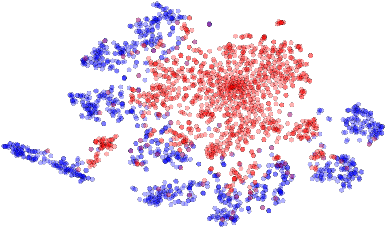
\includegraphics[width=0.45\textwidth]{./figures/adaptation_vis/pool2_mnist2inv_before.pdf}}\hfill%
  \subfigure[Adapted]{%%
    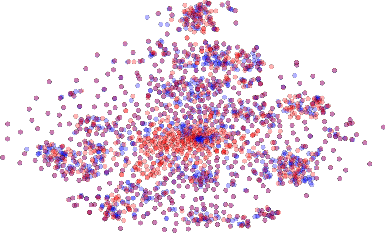
\includegraphics[width=0.45\textwidth]{./figures/adaptation_vis/pool2_mnist2inv_after.pdf}}%%
  \hspace*{\fill}%
  \end{minipage}%
  \begin{minipage}{.5\textwidth}
  \centering
  \small{{\sc Syn Numbers $ \rightarrow $ SVHN}: last hidden layer of the label predictor}
  \setcounter{subfigure}{0}
  \hspace*{\fill}%
  \subfigure[Non-adapted]{%%
    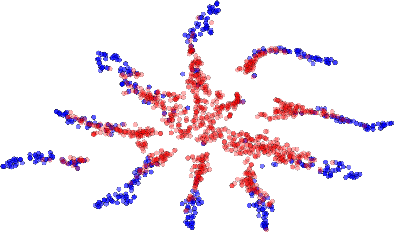
\includegraphics[width=0.45\textwidth]{./figures/adaptation_vis/before.pdf}}\hfill%
  \subfigure[Adapted]{%%
    \includegraphics[width=0.45\textwidth]{./figures/adaptation_vis/after.pdf}}%%
  \hspace*{\fill}%
  \end{minipage}
  \caption{The effect of adaptation on the distribution of the extracted features (best viewed in color). The figure shows t-SNE \cite{Maaten13} visualizations of the CNN's activations {\bf (a)} in case when no adaptation was performed and {\bf (b)} in case when our adaptation procedure was incorporated into training. {\it Blue} points correspond to the source domain examples, while {\it red} ones correspond to the target domain. In all cases, the adaptation in our method makes the two distributions of features much closer.}
  \label{fig:exper_adapt_vis}
\end{figure*}

\subsection{Results}
\label{sect:exper_quant}

We now discuss the experimental settings and the results. In each case, we train on the source dataset and test on a different target domain dataset, with considerable shifts between domains (see \fig{exper_domains_examples}). The results are summarized in \tab{results} and \tab{results_office}. 

\vspace{2mm}\noindent {\bf MNIST $ \rightarrow $ MNIST-M.}
Our first experiment deals with the MNIST dataset~\cite{LeCun98} (source). In order to obtain the target domain ({\sc MNIST-M}) we blend digits from the original set over patches randomly extracted from color photos from BSDS500 \cite{Arbelaez11}. This operation is formally defined for two images $ I^{1}, I^{2} $ as $ I_{ijk}^{out} = | I_{ijk}^{1} - I_{ijk}^{2} | $, where $ i, j $ are the coordinates of a pixel and $ k $ is a channel index. In other words, an output sample is produced by taking a patch from a photo and inverting its pixels at positions corresponding to the pixels of a digit. For a human the classification task becomes only slightly harder compared to the original dataset (the digits are still clearly distinguishable) whereas for a CNN trained on MNIST this domain is quite distinct, as the background and the strokes are no longer constant. Consequently, the source-only model performs poorly. Our approach succeeded at aligning feature distributions (\fig{exper_adapt_vis}), which led to successful adaptation results (considering that the adaptation is unsupervised). At the same time, the improvement over source-only model achieved by subspace alignment (SA) \cite{Fernando13} is quite modest, thus highlighting the difficulty of the adaptation task. 

\vspace{2mm}\noindent {\bf Synthetic numbers $ \rightarrow $ SVHN.}
To address a common scenario of training on synthetic data and testing on  real data, we use Street-View House Number dataset {\sc SVHN} \cite{Netzer11} as the target domain and synthetic digits as the source. The latter ({\sc Syn ~Numbers}) consists of ~500,000 images generated by ourselves from Windows fonts by varying the text (that includes different one-, two-, and three-digit numbers), positioning, orientation, background and stroke colors, and the amount of blur. The degrees of variation were chosen manually to simulate SVHN, however the two datasets are still rather distinct, the biggest difference being the structured clutter in the background of SVHN images. 

The proposed backpropagation-based technique works well covering two thirds of the gap between training with source data only and training on target domain data with known target labels. In contrast, SA~\cite{Fernando13} does not result in any significant improvement in the classification accuracy, thus highlighting that the adaptation task is even more challenging than in the case of the MNIST experiment.

\vspace{2mm}\noindent {\bf MNIST $ \leftrightarrow $ SVHN.}
In this experiment, we further increase the gap between distributions, and test on {\sc MNIST} and {\sc SVHN}, which are significantly different in appearance. Training on SVHN even without adaptation is challenging --- classification error stays high during the first 150 epochs. In order to avoid ending up in a poor local minimum we, therefore, do not use learning rate annealing here. Obviously, the two directions ({\sc MNIST} $ \rightarrow $ {\sc SVHN} and {\sc SVHN} $ \rightarrow $ {\sc MNIST}) are not equally difficult. As {\sc SVHN} is more diverse, a model trained on SVHN is expected to be more generic and to perform reasonably on the MNIST dataset. This, indeed, turns out to be the case and is supported by the appearance of the feature distributions. We observe a quite strong separation between the domains when we feed them into the CNN trained solely on { \sc MNIST}, whereas for the {\sc SVHN}-trained network the features are much more intermixed. This difference probably explains why our method succeeded in improving the performance by adaptation in the {\sc SVHN} $ \rightarrow $ {\sc MNIST} scenario (see \tab{results}) but not in the opposite direction (SA is not able to perform adaptation in this case either). Unsupervised adaptation from MNIST to SVHN gives a failure example for our approach (we are unaware of any unsupervised DA methods capable of performing such adaptation).

\vspace{2mm}\noindent {\bf Synthetic Signs $ \rightarrow $ GTSRB.}
Overall, this setting is similar to the {\sc Syn Numbers} $ \rightarrow $ {\sc SVHN} experiment, except the distribution of the features is more complex due to the significantly larger number of classes (43 instead of 10). For the source domain we obtained~100,000 synthetic images (which we call {\sc Syn~Signs}) simulating various photoshooting conditions. Once again, our method achieves a sensible increase in performance once again proving its suitability for the synthetic-to-real data adaptation.

\begin{figure}
  \centering
  \setlength\figureheight{2.7cm}
  \setlength\figurewidth{6.8cm}
  % This file was created by matlab2tikz v0.5.0 running on MATLAB 8.3.
%Copyright (c) 2008--2014, Nico Schlömer <nico.schloemer@gmail.com>
%All rights reserved.
%Minimal pgfplots version: 1.3
%
%The latest updates can be retrieved from
%  http://www.mathworks.com/matlabcentral/fileexchange/22022-matlab2tikz
%where you can also make suggestions and rate matlab2tikz.
%
\begin{tikzpicture}[font=\scriptsize]

\begin{axis}[%
width=0.95092\figurewidth,
height=\figureheight,
at={(0\figurewidth,0\figureheight)},
scale only axis,
xmin=10000,
xmax=50000,
xlabel={Batches seen},
ymin=0,
ymax=1,
ylabel={Validation error},
axis x line*=bottom,
axis y line*=left,
legend style={at={($ (1,1) + (-0.1cm,-0.1cm) $)},anchor=north east,align=left,legend cell align=left,draw=black},
xmajorgrids,
ymajorgrids,
grid style={dashed}
]
\addplot [color=blue,solid,line width=1.0pt]
  table[row sep=crcr]{%
10500	0.199757996632997\\
11000	0.19162984006734\\
11500	0.190788089225589\\
12000	0.192918771043771\\
12500	0.196390993265993\\
13000	0.185527146464646\\
13500	0.190472432659933\\
14000	0.185606060606061\\
14500	0.183422769360269\\
15000	0.189051978114478\\
15500	0.191524621212121\\
16000	0.186079545454545\\
16500	0.179424452861953\\
17000	0.187684132996633\\
17500	0.187868265993266\\
18000	0.180923821548822\\
18500	0.187315867003367\\
19000	0.178661616161616\\
19500	0.18102904040404\\
20000	0.180555555555556\\
20500	0.176662457912458\\
21000	0.183791035353535\\
21500	0.179214015151515\\
22000	0.178898358585859\\
22500	0.178898358585859\\
23000	0.174479166666667\\
23500	0.174742213804714\\
24000	0.171059553872054\\
24500	0.177951388888889\\
25000	0.174794823232323\\
25500	0.174084595959596\\
26000	0.174636994949495\\
26500	0.169034090909091\\
27000	0.171191077441077\\
27500	0.170875420875421\\
28000	0.171506734006734\\
28500	0.170217803030303\\
29000	0.169244528619529\\
29500	0.169875841750842\\
30000	0.168744739057239\\
30500	0.17048085016835\\
31000	0.169454966329966\\
31500	0.167771464646465\\
32000	0.168849957912458\\
32500	0.168323863636364\\
33000	0.168718434343434\\
33500	0.165667087542088\\
34000	0.167376893939394\\
34500	0.169007786195286\\
35000	0.167140151515152\\
35500	0.165667087542088\\
36000	0.167850378787879\\
36500	0.169823232323232\\
37000	0.170691287878788\\
37500	0.16640361952862\\
38000	0.167981902356902\\
38500	0.169875841750842\\
39000	0.166771885521886\\
39500	0.169376052188552\\
40000	0.168087121212121\\
40500	0.165509259259259\\
41000	0.167718855218855\\
41500	0.168060816498317\\
42000	0.166035353535354\\
42500	0.166692971380471\\
43000	0.166429924242424\\
43500	0.167034932659933\\
44000	0.170349326599327\\
44500	0.169744318181818\\
45000	0.168218644781145\\
45500	0.166429924242424\\
46000	0.166324705387205\\
46500	0.168771043771044\\
47000	0.168034511784512\\
47500	0.168718434343434\\
48000	0.171059553872054\\
48500	0.170638678451178\\
49000	0.16819234006734\\
49500	0.168981481481481\\
50000	0.167902988215488\\
};
\addlegendentry{Real data only};

\addplot [color=cyan,solid,line width=1.0pt]
  table[row sep=crcr]{%
10500	0.9625\\
11000	0.79765625\\
11500	0.715625\\
12000	0.6140625\\
12500	0.52109375\\
13000	0.459375\\
13500	0.4484375\\
14000	0.421875\\
14500	0.39453125\\
15000	0.4109375\\
15500	0.34296875\\
16000	0.36875\\
16500	0.3359375\\
17000	0.36171875\\
17500	0.3171875\\
18000	0.3484375\\
18500	0.32421875\\
19000	0.315625\\
19500	0.346875\\
20000	0.31875\\
20500	0.35390625\\
21000	0.3265625\\
21500	0.33359375\\
22000	0.3171875\\
22500	0.28515625\\
23000	0.30546875\\
23500	0.309375\\
24000	0.2796875\\
24500	0.30859375\\
25000	0.30703125\\
25500	0.3078125\\
26000	0.28671875\\
26500	0.2875\\
27000	0.31484375\\
27500	0.2859375\\
28000	0.29375\\
28500	0.31328125\\
29000	0.3078125\\
29500	0.2859375\\
30000	0.2890625\\
30500	0.284375\\
31000	0.2953125\\
31500	0.26953125\\
32000	0.29921875\\
32500	0.30078125\\
33000	0.2640625\\
33500	0.309375\\
34000	0.2734375\\
34500	0.290625\\
35000	0.26796875\\
35500	0.3015625\\
36000	0.26796875\\
36500	0.2921875\\
37000	0.265625\\
37500	0.2765625\\
38000	0.2859375\\
38500	0.32109375\\
39000	0.28046875\\
39500	0.275\\
40000	0.24921875\\
40500	0.29140625\\
41000	0.26640625\\
41500	0.265625\\
42000	0.259375\\
42500	0.2765625\\
43000	0.26796875\\
43500	0.2765625\\
44000	0.27265625\\
44500	0.25546875\\
45000	0.26484375\\
45500	0.271875\\
46000	0.2703125\\
46500	0.26171875\\
47000	0.246875\\
47500	0.25078125\\
48000	0.29609375\\
48500	0.2640625\\
49000	0.26875\\
49500	0.26015625\\
50000	0.2578125\\
};
\addlegendentry{Synthetic data only};

\addplot [color=red,solid,line width=1.0pt]
  table[row sep=crcr]{%
10500	0.943892045454545\\
11000	0.943892045454545\\
11500	0.943892045454545\\
12000	0.943892045454545\\
12500	0.848300715488216\\
13000	0.658722643097643\\
13500	0.590593434343434\\
14000	0.475484006734007\\
14500	0.313946759259259\\
15000	0.235690235690236\\
15500	0.17879313973064\\
16000	0.152383207070707\\
16500	0.12912984006734\\
17000	0.114478114478114\\
17500	0.116214225589226\\
18000	0.1015625\\
18500	0.10066813973064\\
19000	0.101983375420875\\
19500	0.0914351851851852\\
20000	0.0895675505050505\\
20500	0.0894360269360269\\
21000	0.0827283249158249\\
21500	0.0798611111111111\\
22000	0.0859638047138047\\
22500	0.0799137205387205\\
23000	0.0778619528619529\\
23500	0.0737584175084175\\
24000	0.0742582070707071\\
24500	0.0776778198653199\\
25000	0.0771517255892256\\
25500	0.0725747053872054\\
26000	0.0739425505050505\\
26500	0.0734953703703704\\
27000	0.0730744949494949\\
27500	0.0688920454545455\\
28000	0.0702072811447811\\
28500	0.072337962962963\\
29000	0.0670244107744108\\
29500	0.0733638468013468\\
30000	0.0667613636363636\\
30500	0.0692340067340067\\
31000	0.0652093855218855\\
31500	0.0664720117845118\\
32000	0.0655776515151515\\
32500	0.0671296296296296\\
33000	0.0656039562289562\\
33500	0.0646043771043771\\
34000	0.0668665824915825\\
34500	0.0638678451178451\\
35000	0.065077861952862\\
35500	0.0649989478114478\\
36000	0.0672348484848485\\
36500	0.0668665824915825\\
37000	0.0626052188552189\\
37500	0.0652093855218855\\
38000	0.0626315235690236\\
38500	0.0627893518518518\\
39000	0.0613162878787879\\
39500	0.063236531986532\\
40000	0.0629208754208754\\
40500	0.0639467592592593\\
41000	0.0612899831649832\\
41500	0.0653409090909091\\
42000	0.0608691077441077\\
42500	0.0613425925925926\\
43000	0.0630260942760943\\
43500	0.060106271043771\\
44000	0.0638678451178451\\
44500	0.0602377946127946\\
45000	0.0577388468013468\\
45500	0.062684132996633\\
46000	0.0608164983164983\\
46500	0.0603167087542088\\
47000	0.0577651515151515\\
47500	0.0583175505050505\\
48000	0.0591329966329966\\
48500	0.0607112794612795\\
49000	0.0585805976430976\\
49500	0.0583175505050505\\
50000	0.0590540824915825\\
};
\addlegendentry{Both};

\end{axis}
\end{tikzpicture}%
  \caption{Semi-supervised domain adaptation for the traffic signs. As labeled target domain data are shown to the method, it achieves significantly lower error than the model trained on target domain data only or on source domain data only. \vspace{-4mm}}
  \label{fig:exper_semi_test}
\end{figure}

As an additional experiment, we also evaluate the proposed algorithm for semi-supervised domain adaptation, i.e.\ when one is additionally provided with a small amount of labeled target data. For that purpose we split {\sc GTSRB} into the train set (1280 random samples with labels) and the validation set (the rest of the dataset). The validation part is used solely for the evaluation and does not participate in the adaptation. The training procedure changes slightly as the label predictor is now exposed to the target data. \fig{exper_semi_test} shows the change of the validation error throughout the training. While the graph clearly suggests that our method can be used in the semi-supervised setting, thorough verification of semi-supervised setting is left for future work.


\vspace{2mm}\noindent {\bf Office dataset.} 
We finally evaluate our method on {\sc Office} dataset, which is a collection of three distinct domains: {\sc Amazon}, {\sc DSLR}, and {\sc Webcam}. Unlike previously discussed datasets, {\sc Office} is rather small-scale with only 2817 labeled images spread across 31 different categories in the largest domain. The amount of available data is crucial for a successful training of a deep model, hence we opted for the fine-tuning of the CNN pre-trained on the ImageNet \cite{Jia14} as it is done in some recent DA works \cite{Donahue14,Tzeng14,Hoffman14}. We make our approach more comparable with \cite{Tzeng14} by using exactly the same network architecture replacing domain mean-based regularization with the domain classifier.

Following most previous works, we evaluate our method using 5 random splits for each of the 3 transfer tasks commonly used for evaluation. Our training protocol is close to \cite{Tzeng14,Saenko10,Gong12} as we use the same number of labeled source-domain images per category. Unlike those works and similarly to e.g.\ DLID~\cite{Chopra13} we use the whole unlabeled target domain (as the premise of our method is the abundance of unlabeled data in the target domain). Under this transductive setting, our method is able to improve previously-reported state-of-the-art accuracy for unsupervised adaptation very considerably (\tab{results_office}), especially in the most challenging {\sc Amazon} $ \rightarrow $ {\sc Webcam} scenario (the two domains with the largest domain shift).

\label{sec:conclusion}
We introduce a novel neural network architecture, the Synchronized Spectral CNN (SyncSpecCNN), for semantic annotation on 3D shape graphs. To share coefficients and conduct multi-scale analysis in different parts of a single shape graph, we introduce a spectral parametrization of dilated convolutional kernels. To allow parameter sharing across related but different shapes that may be represented by very different graphs, we introduce a spectral transformer network to synchronize different spectral domains. The effectiveness of different components in our network is validated through extensive experiments. Jointly these contributions lead to state-of-the-art performance on various semantic annotation tasks including 3D shape part segmentation and 3D keypoint prediction.

{\small
\bibliographystyle{ieee}
\bibliography{egbib}
}

\end{document}
